    
\documentclass[reprint, aps, prl, superscriptaddress]{revtex4-2}
\usepackage{graphicx, float, xcolor}
\graphicspath{{fig/}{../../figs/fi_fig/}{../../figs/recover/}}
\usepackage[ruled,linesnumbered]{algorithm2e}
\usepackage{physics}
\usepackage{hyperref}
\usepackage{amsthm, amssymb, bm}
\usepackage[T1]{fontenc}

\let\originalsection\section

\renewcommand{\section}[1]{\par\medskip\noindent\textbf{{\textit{#1.}---}}}
\newcommand{\ii}{\mathrm{i}}
\newcommand{\myqc}{\text{HP}}
\newcommand{\uqc}[1]{U_{\mathrm{HP}}^{(#1)}}
\newcommand{\cpgate}[3]{\mathrm{CP}_{#1, #2}(#3)}
\newcommand{\fii}{\mathrm{DFI}}
\newcommand{\Lambdacomp}[1]{\bar{\Lambda}_{\leq #1}}


\newcommand{\bkm}[1]{\textcolor{cyan}{#1}}

\newtheorem{definition}{Definition}
\newtheorem{theorem}{Theorem}
\newtheorem{proposition}{Proposition}
\newtheorem*{restatedtheorem}{Theorem}
\newtheorem*{restatedproposition}{Proposition}



\begin{document}
\title{$\mathcal{O}(n)$ alternative to Quantum Fourier Transform with efficient neural net classical post-processing}


\author{Kaiming Bian}%12231295@mail.sustech.edu.cn
\thanks{These two authors contributed equally.}
\affiliation{Shenzhen Institute for Quantum Science and Engineering, Southern University of Science and Technology, Shenzhen, 518055, China}
\affiliation{International Quantum Academy, Shenzhen, 518048, China}

\author{Zujin Wen}%zujinwen2-c@my.cityu.edu.hk
\thanks{These two authors contributed equally.}
\affiliation{Department of Physics, City University of Hong Kong, Tat Chee Avenue, Kowloon, Hong Kong SAR, China}
\author{Oscar Dahlsten}
\affiliation{Department of Physics, City University of Hong Kong, Tat Chee Avenue, Kowloon, Hong Kong SAR, China}
\date{\today}

\begin{abstract}
The Quantum Fourier Transform (QFT) is required by hidden subgroup problem (HSP) algorithms, including Shor's algorithm for factoring. The circuit depth of the QFT remains challenging for near-term hardware. To find shallower alternatives we identify two properties that are exploited by the QFT to enable HSP. Firstly, the shift invariance of the QFT allows for the removal of a random overall shift. Secondly, the QFT retains information about the hidden subgroup generator accessible in the measurement outcomes. We quantify that information via the discrete Fisher information. We construct a family of shallow circuits using Hadamards and controlled-Phase gates, HP-$L$ circuits, that we prove preserve shift invariance. Numerical analysis shows these circuits retain exponentially growing Fisher information. The $\mathcal{O}(n)$ HP-$1$ can replace the $\mathcal{O}(n^2)$ QFT in Shor's algorithm, as demonstrated numerically, with an efficient neural network implementing classical post-processing.  
\end{abstract}

\maketitle


\section{Introduction}The $\mathcal{O}(n^2)$ circuit depth required by the standard Quantum Fourier Transform (QFT) presents experimental challenges. The QFT is used in the exponential quantum speedups of landmark protocols—such as Shor's algorithms for prime factorization and discrete logarithms \cite{Simon1997, Shor1994, Shor1997}. The associated family of algorithms, all using the QFT, is known as the (quantum) hidden subgroup problem (HSP) algorithms \cite{Kitaev1995, Jozsa2001, Lomont2004, liu2024information}. The experimental implementation of the QFT remains challenging. For a $100$-qubit system ($n=100$), the QFT demands thousands of circuit layers, which vastly exceeds current hardware capabilities. For instance, IBM's $127$-qubit Eagle processor is limited to a depth of $60$ layers even with extensive error mitigation \cite{kim2023evidence}; Google's $105$-qubit Willow processor reaches its operational threshold at around $40$ layers~\cite{google2025quantum}; USTC's $105$-qubit Zuchongzhi~3.0 processor demonstrated random circuit sampling on $83$-qubits, with around $32$ layers~\cite{Zuchongzhi}. Moreover, for quantum error-mitigation protocols that are commonly used, the sampling overhead can scale exponentially with the circuit depth~\cite{takagi2022fundamental, takagi2023universal}.


There has been significant progress in reducing the circuit depth required. These efforts have enabled record experimental QFT fidelities \cite{aumann2026demonstrating} through techniques including (i) approximate or truncated QFT constructions, which omit small-angle controlled rotations \cite{Coppersmith2002, park2023reducing} with \(\mathcal{O}(n\ln n)\) depth, (ii) dynamic mid-circuit measurements, which reduce the resource scaling of QFT followed immediately by measurement from \(\mathcal{O}(n^2)\) two-qubit gates to \(\mathcal{O}(n)\) mid-circuit measurements without connectivity constraints \cite{baumer2024quantum}, and (iii) quantum circuit cutting and cluster-simulation methods, which trade coherent quantum depth for additional sampling and classical post-processing overhead~\cite{tang2021cutqc, Peng2020}. 

We here take a different approach to reducing the circuit depth required. Rather than approximate the QFT we identify key features of the QFT that make it compatible with the HSP. We focus on shift-invariance combined with retention of information about the generator in question. Fig.~\ref{fig:illus}(a) summarizes the main idea. We design non-QFT circuits that retain those key features. 


\begin{figure}[htbp]
    \centering
    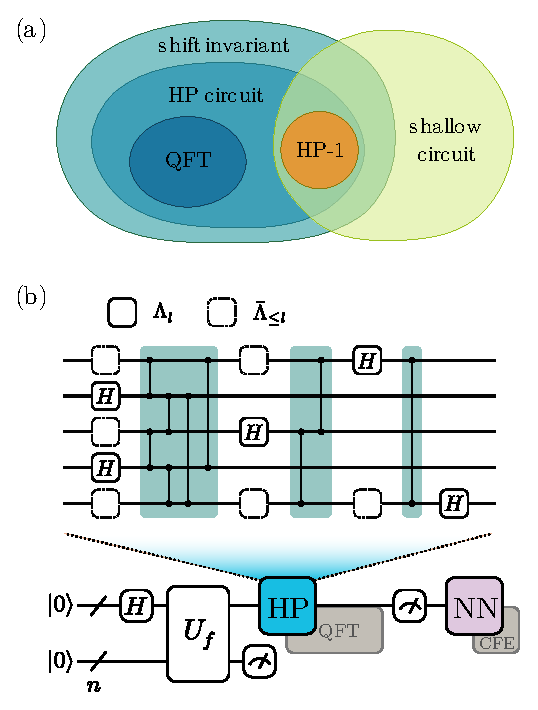
\includegraphics[width=0.8\columnwidth]{illus v1.4.pdf}
    \caption{\label{fig:illus} \textbf{Shallow shift-invariant alternative to the QFT.} (a) Shift invariance is a critical property of the QFT. We design a circuit family, denoted as \myqc-$L$, that preserves the shift invariance. Within this broader family, \myqc-1 specifically serves as a shallow-depth circuit that is experiment-friendly. (b) In the proposed HSP algorithmic routine, the deep QFT block (the left gray gate) is directly replaced by the \myqc~circuit. A neural network then processes the measurement outcomes, bypassing the standard continued fraction expansion (CFE) typically used in the standard HSP. The HP circuit is composed of Hadamard and phase gates, with $\Lambda_l$ referring to the qubits with Hadamards applied in layer $l$. }
\end{figure}


We construct a circuit family, called \myqc-$L$ circuits, that preserves shift invariance. In particular, the \myqc-$1$ circuits are shallow and retain information about the generator. The \myqc-$L$ circuits interleave transversal Hadamard (H) gates with $L$ layers of phase (P) blocks. We prove analytically that \myqc-$L$ circuits are shift-invariant. Numerical scaling analysis demonstrates exponentially increasing retention of Fisher information $\sim e^{kn}$, albeit with a worse exponent $k$ than QFT. That $\sim e^{kn}$-scaling consistent with efficient scaling of the number of samples required. 

We numerically simulate replacing the QFT in Shor's algorithm with \myqc-1 circuits, and using an efficiently scaling neural network~\cite{zaheer2017deep} for classical post-processing. Factorisation is successfully achieved.  

\section{Necessary condition for Shift Invariance}The standard quantum HSP algorithm is illustrated in Fig.~\ref{fig:illus}(b) with gray blocks \cite{Shor1994, Shor1997, Simon1997, Jozsa2001}.
After $U_f$, the state is proportional to $\sum_x \ket{x}\ket{f(x)}$. The elements $x$ belong to a finite abelian group $G$ with group operation +. We are guaranteed that $f(x+r)=f(x)$ for the unknown generator $r$ that we wish to find. In other words, the function $f(\cdot)$ is constant on cosets of $V$, the subgroup generated by $r$. Upon measuring (or imagining measuring) the second register to find $\ket{f(c)}$ the state becomes proportional to $\sum_{q\in \{0,1,2...\}} \ket{c+qr}\ket{f(c)}$, where the shift $c$ acts as a random coset offset and does not affect the recovery of $r$ (additional details about the HSP algorithm are provided in
Appendix~\ref{append: hsp and fs}).

We now define shift invariance~\cite{NielsenChuang2000} for HSP sampling and derive a necessary condition that any shift-invariant unitary must satisfy. For a subgroup $V \le G$, in particular $V=\{\ket{qr}\}$, we denote the uniform superposition over its elements as $\ket{V} := \sum_{q\in \{0,1,2...\}} \ket{qr}  = \frac{1}{\sqrt{|V|}} \sum_{v \in V} \ket{v}$, for notational simplicity.

\begin{definition}[Shift invariance]
    % Let $T_c\ket{v} = \ket{v + c}$ be the shift operator for $c \in G$. 
    A unitary $U$ acting on the group register is shift-invariant for HSP sampling if
    \begin{equation}
    \label{eq:shift invariant def}
        \left|\bra{x}U\ket{V}\right|^2
        =
        \left|\bra{x}U \ket{c+V}\right|^2,
        ~~
        \forall x,c \in G,\ \forall V \le G.
    \end{equation}
\end{definition}

To identify shift-invariant circuits beyond the QFT, we first establish a necessary condition for shift invariance.
\begin{proposition}[Necessary condition of shift invariance]
\label{thm:necessary_modulus_condition}
    Suppose $U$ is a unitary on the group register that satisfies the shift-invariance condition above. Then, for every $x,y\in G$ there exist phases $\theta_{xy}\in\mathbb{R}$ such that
%    \begin{equation}
        %\left|\bra{x}U\ket{y}\right|=\frac{1}{\sqrt{|G|}}.
    %\end{equation}
    \begin{equation}
        \bra{x}U\ket{y}=\frac{1}{\sqrt{|G|}}e^{\ii\theta_{xy}}.
    \end{equation}
\end{proposition}

\begin{proof}[Proof sketch of Proposition~\ref{thm:necessary_modulus_condition}]
The proof hinges on analyzing the shift-invariance condition for the trivial subgroup $V = \{0\}$. For $V = \{0\}$, the state $\ket{V}$ is the computational basis state $\ket{0}$, and the shifted state is $\ket{c+V} = \ket{c}$. The requirement (Eq.\eqref{eq:shift invariant def}) that $\left|\bra{x}U\ket{0}\right|^2 = \left|\bra{x}U\ket{c}\right|^2$ for all $x, c \in G$ implies that, for any fixed output $x$, the magnitude of every matrix element in the $x$-th row of $U$ must be identical. The special case induces the uniform magnitude $\bra{x}U\ket{y} = 1/\sqrt{|G|} e^{\ii \theta_{xy}}$. The full details of this argument are provided in Appendix~\ref{app:necessary condition of sinv}.
\end{proof}

\section{L-phase-block Hadamard-Phase circuits (\myqc): A shift-invariant circuit family}Proposition \ref{thm:necessary_modulus_condition} suggests a simple design principle for constructing shift-invariant circuits. The condition \(|\langle x|U|y\rangle|=1/\sqrt{|G|}\) requires flat amplitude magnitudes, which are naturally generated by Hadamard gates. The remaining freedom lies in the relative phases \(\theta_{xy}\), which can be adjusted by controlled-phase gates ($\mathrm{CP}(\theta)=\ket{00}\bra{00}+\ket{01}\bra{01}+\ket{10}\bra{10}+e^{\ii\theta}\ket{11}\bra{11}$) without changing these magnitudes. This motivates the Hadamard-phase (HP) circuit family we shall now introduce. As illustrated in Fig.~\ref{fig:illus} (b), the \myqc-$L$ circuit is structured as an alternating sequence of Hadamard gates and phase blocks. To respect shift invariance, we enforce three rules for \myqc-$L$: (i) each qubit is acted on by a Hadamard gate exactly once; (ii) each qubit pair is connected by at most one controlled-phase gate; and (iii) each controlled-phase gate must come together with 2 Hadamards, one before and one after the phase gate. Here, ``once'' refers to the entire $L$-layer circuit rather than to a single layer. 


To express the allowed circuits mathematically, we define two types of sets of qubits.
Let \(H_i\) denote the Hadamard gate applied to qubit
\(i\in\{1,2,\ldots,n\}\). For each layer \(l\), let
\(\Lambda_l\) denote the set of qubits on which
Hadamard gates are applied in that layer. The qubits that are still allowed in terms of having a Hadamard on them after layer $l$, i.e.\ those that have not had a Hadamard on them in or before layer $l$, are denoted as the set \(\Lambdacomp{l}\).

In-between the Hadamard layers, the two sets are coupled via a controlled-phase block, denoted as $\cpgate{\Lambda_l}{\Lambdacomp{l}}{\bm{\theta}_{\Lambda_l\Lambdacomp{l}}}$, which applies pairwise operations $\mathrm{CP}_{jk}(\theta_{jk})$ between each qubit $j \in \Lambda_l$ and $k \in \Lambdacomp{l}$. Building upon this notation, we formally define the circuit architecture:
\begin{definition}[\myqc-$L$ circuit]
    A quantum circuit is classified as an \myqc-L circuit if it is constructed using the following layer-wise architecture
    \begin{equation}
    \label{eq:HP}
        \uqc{L}({\bm{\theta}}) = \bigotimes_{i \in \Lambda_L} H_{i}\prod_{l=L-1}^{1} \left( \cpgate{\Lambda_l}{\Lambdacomp{l}}{\bm{\theta}_{\Lambda_l\Lambdacomp{l}}} \bigotimes_{i \in \Lambda_l} H_{i} \right),
    \end{equation}
    where the controlled-phase block is given by
    \begin{equation}
        \cpgate{\Lambda_l}{\Lambdacomp{l}}{\bm{\theta}_{\Lambda_l\Lambdacomp{l}}} = \prod_{j \in \Lambdacomp{l}} \prod_{k \in \Lambda_l} \mathrm{CP}_{jk}(\theta_{jk}).
    \end{equation}
    The parameter set $\bm{\theta}_{\Lambda_l\Lambdacomp{l}}$ is the collection of $\theta_{jk}$, $j\in \Lambda_l$, $k \in \Lambdacomp{l}$. 
\end{definition}


    
In the following, we show that HP circuits preserve shift invariance. This implies that such invariance is not unique to the QFT, but is a feature that arises in a wider family of quantum circuits. 


\begin{theorem}
\label{thm:hp_circuits_are_sinv}
    \myqc-$L$ circuits are shift-invariant for $\mathbb{Z}_{2^{n}}$.
\end{theorem}
The proof involves giving an analytical expression for the state evolved under an HP-L circuit (Eq.\eqref{eq:HP}) and checking that shift invariance is indeed respected (Appendix~\ref{app:HPk are sinv}).



% \section{\myqc-0 can be used in HSP over $\mathbb{Z}_{2^n}$}We give an analytical solution for HSP over $\mathbb{Z}_{2^n}$ via parallel Hadamard gates. We consider the cyclic group $\mathbb{Z}_{2^n}$ since the group can be naturally represented in the computational basis. In this case, each subgroup is generated by a power of two,
% \begin{equation}
%     V=\{q2^p:q=0,\ldots,2^{n-p}-1\} \leq \mathbb{Z}_{2^n},
% \label{eq: hp0 subgroup}
% \end{equation}
% where \(p\) specifies the subgroup generator \(2^p\). Applying a transversal Hadamard layer to a coset state gives
% \begin{equation}
%     H^{\otimes n}\ket{c+V}
%     \propto
%     \sum_{k\in\{0,1\}^{p}}(-1)^{k\cdot c}\ket{0}^{\otimes(n-p)}\ket{k}.
%     \label{eq: hp0 after th}
% \end{equation}
% By measuring the state $H^{\otimes n}\ket{c+V}$, one observes that the first $n-p$ bits are always fixed to 0, while the remaining $p$ bits are uniformly distributed over $\{0,1\}^p$. Thus, the value of $p$ can be determined by identifying which bit positions are consistently zero. The detailed calculation and sampling algorithm are provided in Appendix~\ref{app:transversal_hadamard_sampling}.



\section{\myqc-$L$ for HSP over $\mathbb{Z}$: information on generator is retained}
For HSP over $\mathbb Z_{2^n}$, \myqc-0, namely a parallel Hadamard layer,
gives an analytically solvable recovery procedure for the hidden subgroup
generator $2^p$. The key observation is that the first $n-p$ measurement bits
are deterministically zero after applying $H^{\otimes n}$ to a coset state,
allowing $p$ to be read off from the zero pattern; the full calculation and
sampling algorithm are given in
Appendix~\ref{app:transversal_hadamard_sampling}. However, the protocol $\myqc$-0 fails for general cyclic groups $\mathbb{Z}_q$ because the measurement distributions corresponding to different subgroups $V$ are not distinguishable. That absence of distinguishability demonstrates that shift invariance alone is insufficient for successful hidden subgroup recovery, and that distinguishability should be imposed as an additional condition. 

\begin{figure}[t]
    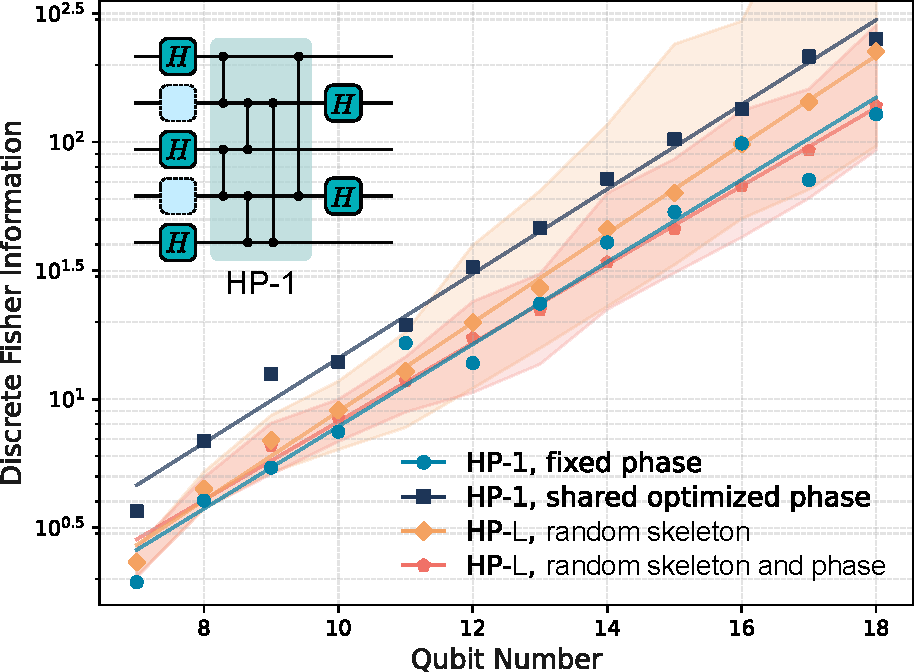
\includegraphics[width=0.45  \textwidth]{fi_fig v3.pdf}
    \caption{\label{fig:fi_scaling} 
\textbf{Average discrete Fisher information (DFI) increasing with the number of qubits.} Results are shown for several HP-family circuit settings. $L$ denotes the number of phase blocks layers with HP-1 having a single phase block layer.  Solid curves show the mean, with shaded bands indicating one standard deviation associated with random phase choices.}


    
\end{figure}


We use the discrete Fisher information (DFI) as a metric for distinguishability.
\begin{equation}
\label{eq:DFI}
    \fii(r, n) = \sum_{x = 0}^{2^n -1} \frac{\left(\text{Pr}(x\mid r+1) - \text{Pr}(x\mid r)\right)^2}{\text{Pr}(x\mid r)},
\end{equation}
where $x$ represents measurement outcomes, $r$ is the hidden subgroup generator, and $\text{Pr}(x\mid r)$ is the probability of measuring $x$ when the subgroup generator is $r$. 



% Original eq. 8 
% The sample complexity for estimating a discrete parameter is formally governed by the DFI (Eq.\eqref{eq:DFI}) via the Hammersley-Chapman-Robbins bound~\cite{chapman1951minimum, hammersley1950estimating}, 
% \begin{equation}
%     m \ge \frac{\ln\left( 1 + \epsilon^{-2} \right)}{\ln\left( 1 + \fii(r) \right)},
% \end{equation}
% where $m$ is the required number of samples and \(\epsilon\) denotes the maximum tolerable standard deviation of the estimator of the parameter. The bound suggests that retaining an exponentially growing DFI results in tractable ($m$ lower-bounded by $o(\frac{1}{n}$)) sample complexity for the subsequent neural-network-based post-processing. 


For the standard QFT (Appendix~\ref{app:qft_fisher_information}), we can calculate the DFI as
\begin{equation}
\label{eq:qft dfi}
    \fii_{\mathrm{QFT}}(r,n) \approx \frac{4\pi^2}{9}\left(\frac{2^{2n}}{r^2}-1\right) \sim \mathcal{O}\left(2^{2n}\right).
\end{equation} 
Eq.~\eqref{eq:qft dfi} indicates that the generator $r$ becomes easier to recover as the qubit number increases, which motivates us to limit $r$ to $1 \ll r \ll 2^n$. 

% newly added theorem 2 and 3
For \myqc-1, Lemma~\ref{lem:hp1_c_twisted_numerator} gives the
\(C\)-twisted dyadic-resonance scaling of the adjacent-period numerator.  The
resulting numerical Fisher-information scan is summarized by the following
ln-linear law.

\begin{theorem}[Ln-linear minimum Fisher information for \myqc-1]
\label{thm:hp1_first_order_fisher_transfer_maintext}
For \myqc-1, restrict the adjacent-period scan to generators satisfying
\(r^2\ll 2^n\).  The minimum adjacent-period DFI obeys the ln-linear scaling
\begin{equation}
    \ln \fii_{\min}(n)\sim kn+b,
    \label{eq:hp1_fisher_ln_linear_minimum}
\end{equation}
\end{theorem}

The proof of this theorem relies on a statistical regularity of the amplitudes: the contribution of \(\langle x|U|V\rangle\), with \(V=\langle r\rangle\), to the adjacent probability change \(\text{Pr}(x\mid r+1)-\text{Pr}(x\mid r)\) is governed primarily by the scale of \(r\).
Theorem~\ref{thm:hp1_first_order_fisher_transfer_maintext} shows that, within the square-root resolvability window, \myqc-1 circuits retain exponentially growing information about the hidden subgroup generator.

The same distinguishability mechanism also gives a statistical separation guarantee beyond the local Fisher-information criterion. 
For two adjacent output distributions \(P_r\) and \(P_{r+1}\), define the Chernoff information as
\begin{equation}
    \mathcal C(P_r,P_{r+1})
    :=
    -\ln \min_{0\leq \alpha\leq 1}
    \sum_x P_r(x)^\alpha P_{r+1}(x)^{1-\alpha}.
\end{equation}

\begin{theorem}[Chernoff separation of \myqc-1]
\label{thm:hp1_chernoff_poly_bound}
Assume the same \(C\)-twisted dyadic-resonance scaling heuristic as in
Lemma~\ref{lem:hp1_c_twisted_numerator}. 
If \(r\le n^a\) for a fixed constant \(a\), then
\begin{equation}
    \mathcal C(P_r,P_{r+1})
    \ge
    \frac{1}{\operatorname{poly}(n)}.
    \label{eq:hp1_chernoff_inverse_polynomial}
\end{equation}
More generally, the same conclusion holds whenever
\(r\operatorname{poly}(n)=o(e^{kn+b})\).
\end{theorem}

Thus, adjacent generators are separated not only in the DFI sense, but also in terms of statistical distinguishability.








For \myqc{} circuits, the DFI is evaluated numerically. Specifically, for a fixed $r$, the circuit maps the periodic input components $\{\ket{qr}\}_q$ to a computational-basis distribution over outcomes $\ket{b}$, with the exact probabilities given by $\mathrm{Pr}(\ket{b}) = \left|\sum_q \langle b|U|qr\rangle\right|^2$.
To evaluate the worst-case parameter sensitivity as the system scales, we consider the 
worst-case DFI: $\fii_{\min}(n):=\min_{2 \leq r \leq 2^{n/2}} \fii(r,n)$.
Fig.~\ref{fig:fi_scaling} illustrates the minimum DFI against the qubit number $n$. (We bound the period by the square-root resolvability scale $r\le 2^{n/2}$, which keeps $r \ll 2^n$.)

Fig.~\ref{fig:fi_scaling} also compares the scaling of different \myqc~circuit configurations, where solid curves and shaded bands represent the mean and standard deviation of $\fii_{\min}(n)$. The fixed-phase \myqc-1 circuit utilizes the skeleton, $\Lambda_1 = \{1,3,5, \cdots\}$ and $\Lambda_2 = \{2,4,6, \cdots\}$, with controlled-phase gates with phase $\frac{2\pi}{2^{|i-j|}}$ between qubits $i$ and $j$. The optimized \myqc-1 circuit adopts the same skeleton but treats the gate phases as variational parameters, trained to maximize the $\fii_{\min}$. The deeper \myqc{}-$L$ circuits are constructed by generating valid random skeletons $\Lambda$. 


The proposed \myqc~circuit family preserves an exponential growth trend of DFI over this square-root period window. Appendix~\ref{app:fi_ln_linear_growth} reports the corresponding ln-linear regression coefficients.






\begin{figure}[!t]
    \centering
    \makebox[\columnwidth][l]{\textbf{(a)}}\\[-0.2em]
    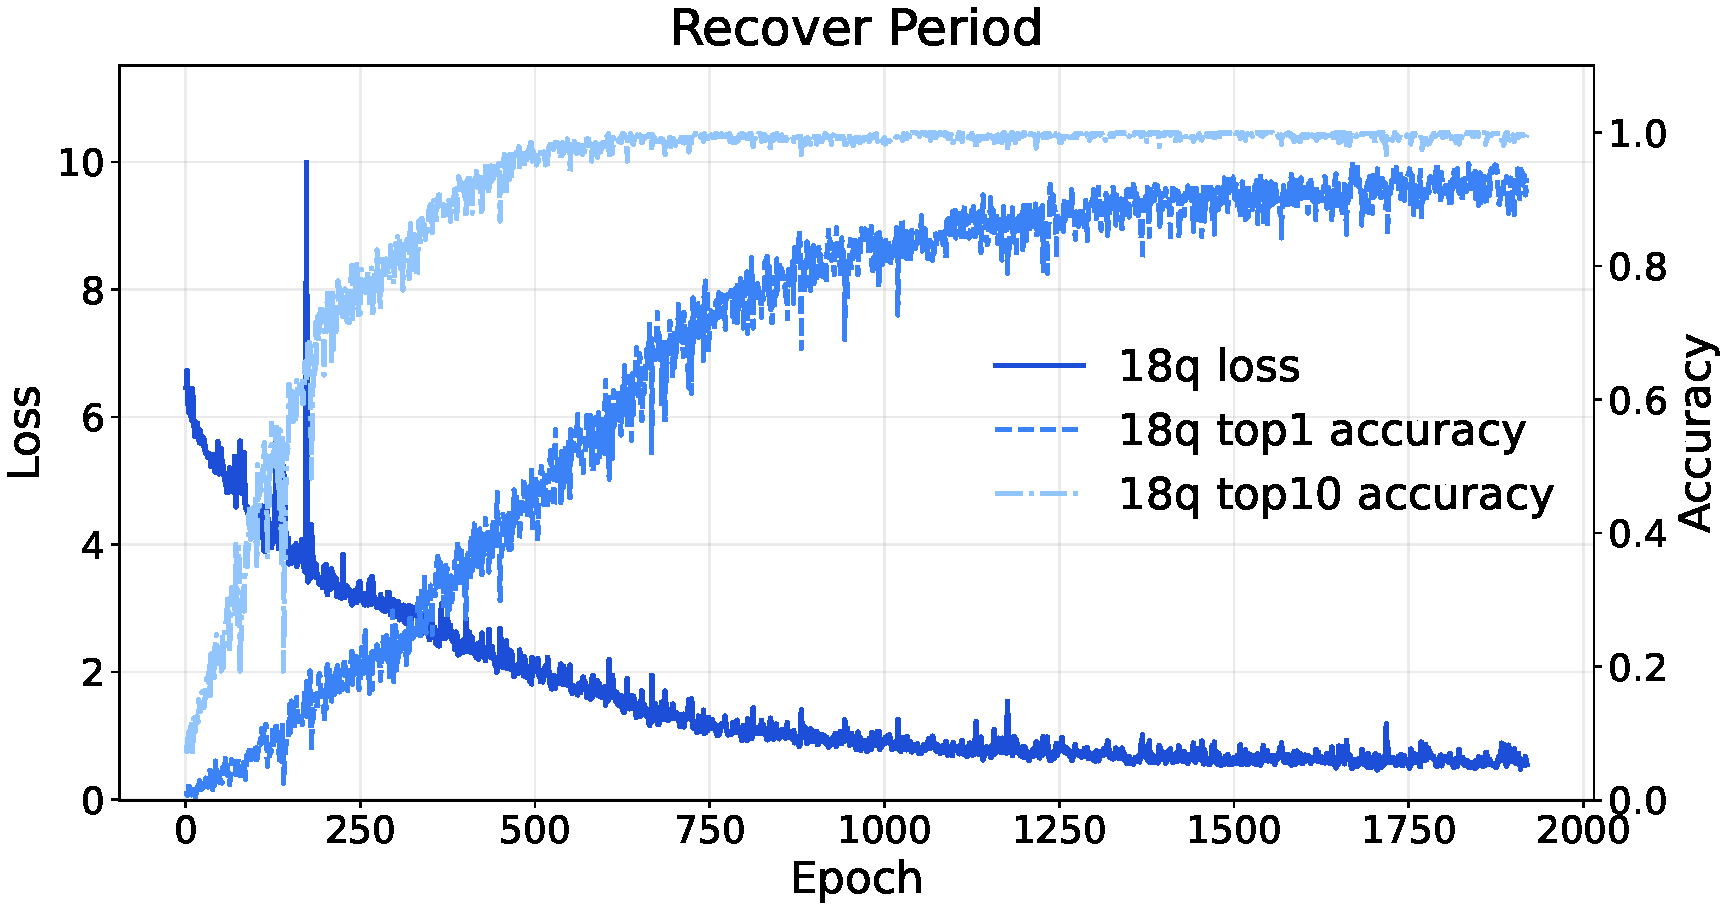
\includegraphics[width=\columnwidth]{period_recovery_18q_val_metrics.pdf}
    \vspace{0.5em}
    \makebox[\columnwidth][l]{\textbf{(b)}}\\[-0.2em]
    \includegraphics[width=\columnwidth]{shor_foundk_overview.pdf}
    \caption{\label{fig:recovery_pipeline}
    \textbf{Numerical simulation shows successful Shor factoring via \myqc-1 and neural net post-processing.}
    (a) Validation loss, top-1 accuracy, and top-10 accuracy for neural-network period recovery on an 18-qubit instance.
    (b) Shor-type factorization on 18-qubit semiprime instances with \(N=225001,\ldots,254999\). Colour indicates the minimum number \(k\) of HP-\(1\)-based guesses needed for successful factorization, and grey entries indicate cases where no valid base $a$ yields a detectable period within the chosen bound.
}
\end{figure}

\section{Efficient neural network for classical post-processing}To avoid the exponential costs associated with processing full probability distributions, we employ a poly($n$) Deep Sets neural network \cite{zaheer2017deep, edwards2016towards} to predict the hidden subgroup generator directly from the raw measurement outcomes $\{b_i\}$. The input data is generated using the optimized \myqc-1 circuit evaluated in Fig.~\ref{fig:fi_scaling}. 

The outcomes are fed into a shared feature map \(\phi\), which maps each bitstring \(b_i\) to a feature vector within 2 linear layers and $16n$ feature dimension. The feature vectors are then summed to form an aggregated, permutation-invariant representation $\sum_i\phi(b_i)$. Subsequently, a beam-search decoder \cite{sutskever2014sequence, wiseman2016sequence} performs a top-$k$ search to rank candidate periods. We use polynomial samples $m = 1024n^2$ to train the neural net. This architecture avoids exponential sample-space computations and outputs a ranked list of candidate generators for classical verification.

\section{Replacing \texorpdfstring{$\mathcal{O}(n^2)$}{O(n2)} QFT with \texorpdfstring{$\mathcal{O}(n)$}{O(n)}\myqc{}-1 in Shor's Algorithm}We evaluate the optimized \myqc{}-1 circuit in classical numerical simulations of Shor's algorithm for factoring with neural net classical post-processing. Shor's algorithm seeks the generator $r$ satisfying $a^r \equiv 1 \pmod{N}$. We select the base $a$ such that $1 \le r \le 2^{n/2}$, ensuring resolvability by the $n$-qubit register. We consider factoring 18-qubit semiprime instances with \(N=225001,\ldots,254999\).

The neural net trained successfully. As shown in Fig.~\ref{fig:recovery_pipeline}(a), the neural network achieves rapid convergence when trained on an 18-qubit instance. Both the top-1 (correct period ranked first) and top-10 accuracies increase swiftly within a few epochs.

The combined HP-1 and neural net protocol recovers the subgroup generator in the tested instances. As illustrated in Fig.~\ref{fig:recovery_pipeline}(b), each composite integer is colored by the minimum number of guesses $k$. Most solved instances are solved on the first attempt ($k=1$), and the remaining solved instances require $k=2$. 

Noise simulation under a post-circuit global depolarizing channel demonstrates that our protocol with the optimized \myqc-1 circuit is robust against moderate environmental noise. The recovery accuracy remains stable up to noise-strength $\eta \approx 0.215$ for $10$ qubits ($1-\eta$ is the probability of applying the identity to the input state). Appendix~\ref{app:noise_robustness_details} provides detailed settings, complete numerical results, and corresponding interpretations.

\section{Summary and outlook}We propose a hardware-efficient framework for solving the HSP by shallow, shift-invariant \myqc{}-1 circuits with a polynomial-scaling neural network. To verify the scalability of this protocol, we analyzed the growth model of the DFI. Finally, we evaluated our protocol on Shor's algorithm. The numerical simulations demonstrate that our approach successfully finds the hidden subgroup with high accuracy and remains robust against moderate depolarizing noise.

Realizing a practical HSP protocol further requires optimized implementations of the oracle $U_f$.
Related strategies for reducing oracle and data-loading costs include Hamiltonian-learning-based state preparation that transfers the cost to classical preprocessing and uses \(\mathcal{O}(1)\) oracle queries \cite{learning_hamiltonian_2025}, space-time tradeoffs for non-Clifford gate reductions \cite{yu2025back}, and automatic oracle synthesis frameworks \cite{aos_qdk_2024}. 

Apart from the $\mathcal{O}(n)$ scaling being hardware friendly, the reduction to grouped phase gates in \myqc~circuits makes the phase operations easier to implement than individual phase gate execution. This hardware-level efficiency arises because consecutive phase operations can be merged into single continuous pulses across multiple experimental platforms, including in linear optics \cite{carolan2015universal, Kok2007}, neutral-atom systems \cite{saffman2010quantum, evered2023high, mohan2025parametrized}, trapped ions \cite{Leibfried2003, Tan2013}, and NMR \cite{vandersypen2004nmr}.

\section{Acknowledgements}We acknowledge support from The Guangdong Provincial Quantum Science Strategic Initiative (Grant No. GDZX2503001) and the City University of Hong Kong (Proj. 9610623).
\section{Code Availability}All code relevant to this work is publicly available in the GitHub repository: \url{https://github.com/Fragecity/altqft}.

\bibliography{ref.bib}
\onecolumngrid
\allowdisplaybreaks
\let\section\originalsection
\appendix
\setcounter{secnumdepth}{1}

\makeatletter
\@ifundefined{lemma}{\newtheorem{lemma}{Lemma}}{}
\makeatother


\section*{Appendix}
\makeatletter
\def\@sectioncntformat#1{\csname the#1\endcsname.\quad}
\def\@hangfrom@section#1#2#3{#1#2#3}
\makeatother



\section{Hidden Subgroup Problem and Fourier Sampling}
\label{append: hsp and fs}
% In this section, we outline the standard method for solving the Hidden Subgroup Problem (HSP) over finite abelian groups \cite{Kitaev1995,Jozsa2001,Lomont2004}. Formally, the HSP is defined as follows:

For completeness, this section reviews the standard quantum algorithm for solving the Hidden Subgroup Problem (HSP) over finite abelian groups \cite{Kitaev1995,Jozsa2001,Lomont2004}. Formally, the HSP is defined as follows:

\begin{definition}[Hidden Subgroup Problem]
    Given a function $f: G \to X$ defined on a group $G$, with the promise that there exists a hidden subgroup $V \leq G$ such that for all $g_1, g_2 \in G$
    \begin{equation}
        f(g_1) = f(g_2) \Longleftrightarrow g_1 - g_2 \in V
    \end{equation}
    The objective of this task is to identify the hidden subgroup $V$.
\end{definition}

In the context of this paper, we restrict our attention to finite abelian groups. For such groups, the fundamental theorem of finite abelian groups allows us to express the group structure as a direct product of cyclic groups:
\begin{equation}
    G \cong \mathbb{Z}_{p_1} \times \mathbb{Z}_{p_2} \times \cdots \times \mathbb{Z}_{p_k}.
\end{equation}

The standard quantum procedure for solving the hidden subgroup problem begins by preparing a uniform superposition over all elements of the group $G$ \cite{Kitaev1995,NielsenChuang2000}. We initialize the system in the state
\begin{equation}
    \ket{\psi} = \frac{1}{\sqrt{|G|}} \sum_{g \in G} \ket{g} \ket{0},
\end{equation}
where $|G|$ is the number of elements of the group $G$. The first register holds the group elements, and the second register is initialized to a standard basis state. Next, we evaluate the quantum oracle corresponding to the function $f$, which acts on the two registers and entangles the group elements with their corresponding function values
\begin{equation}
    \ket{\psi} = \frac{1}{\sqrt{|G|}} \sum_{g \in G} \ket{g} \ket{f(g)}.
\end{equation}

% Since the function $f$ is constant on the cosets of the hidden subgroup $H$ and distinct on different cosets, it is highly advantageous to group the terms in the superposition according to these cosets. 

Grouping the superposition terms according to cosets is illuminating, as the function $f$ is constant within each coset of the hidden subgroup $V$ and distinct across different cosets.

Before proceeding, it is useful to formalize the state notation for a subset. For any subset $S \subseteq G$, we define its corresponding normalized quantum state $\ket{S}$ as the uniform superposition over all elements within the set:
\begin{equation}
    \ket{S} = \frac{1}{\sqrt{|S|}} \sum_{s \in S} \ket{s}.
\end{equation}
Using this definition, the normalized state for a specific coset $c+V$ is directly given by
\begin{equation}
    \ket{c+V} = \frac{1}{\sqrt{|V|}} \sum_{v \in V} \ket{c+v}.
\end{equation}

By applying this coset state definition, the post-oracle state can be elegantly rewritten as a superposition of these orthogonal coset states, each perfectly entangled with its unique function evaluation:
\begin{equation}
    \ket{\psi} = \sqrt{\frac{|V|}{|G|}} \sum_{c\in C} \ket{c+V} \ket{f(c)},
\end{equation}
where $C$ is the set of all possible coset representatives. For simplicity, we assume that the second register is measured immediately after the oracle query. Measuring the second register yields a specific outcome $f(c)$ with a uniform probability of $|V|/|G|$. Consequently, the first register collapses into the corresponding pure coset state:
\begin{equation}
    \ket{\psi_{\text{post}}} = \ket{c+V}.
\end{equation}
From this point forward, our analysis will focus exclusively on the quantum state of this first register.

% These two descriptions are different at the state level, but they induce the same Fourier-basis statistics because every coset state has the same measurement distribution after the quantum Fourier transform.
Whether the second register is physically measured to collapse the first register into a pure coset state $\ket{c+V}$, or traced out to leave it in a mixed state, the resulting Fourier-basis statistics remain identical \cite{NielsenChuang2000}. The quantum Fourier transform produces a measurement distribution that is independent of the coset representative. For simplicity, we assume the second register is measured immediately after the oracle query, allowing our subsequent analysis to focus exclusively on the pure coset state:
\begin{equation}
    \ket{\psi_{\text{post}}} = \ket{c+V}.
\end{equation}


A direct measurement in the computational basis is uninformative. Indeed, using the definition of the coset state,
\begin{equation}
    \langle g|c+V\rangle
    = \frac{1}{\sqrt{|V|}} \sum_{v \in V} \langle g|c+v\rangle
    = \frac{1}{\sqrt{|V|}} \sum_{v \in V} \delta_{g,c+v}.
\end{equation}
For fixed $c$, the map $v \mapsto c+v$ is a bijection from $V$ to the coset $c+V$. Therefore the sum $\sum_{v \in V} \delta_{g,c+v}$ equals $1$ when $g \in c+V$ and equals $0$ when $g \notin c+V$. Hence
\begin{equation}
    \Pr[g\,|\,c,V] = |\langle g|c+V\rangle|^2 =
    \begin{cases}
        1/|V|,& g\in c+V,\\
        0,& g\notin c+V,
    \end{cases}
\end{equation}
so the observed element is uniform on the unknown coset. Averaging over uniformly random cosets gives the marginal distribution
\begin{equation}
    \Pr[g]=\frac{1}{|G|},
\end{equation}
which contains no direct information about the hidden subgroup $V$.

To extract meaningful information, we must apply the QFT over the group $G$ before measuring \cite{Kitaev1995,Jozsa2001}. Let $\chi_y(g)$ denote the group characters. The QFT maps a computational basis state $\ket{g}$ as follows:
\begin{equation}
    \text{QFT} \ket{g} = \frac{1}{\sqrt{|G|}} \sum_{y \in G} \chi_y(g) \ket{y}.
\end{equation}
Applying this transformation to our pure coset state $\ket{c+V}$ yields:
\begin{align}
    \text{QFT} \ket{c+V} &= \frac{1}{\sqrt{|V|}} \sum_{h \in V} \text{QFT} \ket{c+v} \nonumber \\
    &= \frac{1}{\sqrt{|V||G|}} \sum_{v \in V} \sum_{y \in G} \chi_y(c+v) \ket{y} \nonumber \\
    &= \frac{1}{\sqrt{|V||G|}} \sum_{y \in G} \chi_y(c) \left( \sum_{v \in V} \chi_y(v) \right) \ket{y}.
\end{align}
By the orthogonality of group characters, the sum $\sum_{v \in V} \chi_y(v)$ evaluates to $|V|$ if the character $\chi_y$ is trivial on $V$ (i.e., $y$ belongs to the orthogonal subgroup $V^\perp$), and evaluates to $0$ otherwise. Thus, the state simplifies to a superposition over $V^\perp$:
\begin{equation}
    \text{QFT} \ket{c+V} = \sqrt{\frac{|V|}{|G|}} \sum_{y \in V^\perp} \chi_y(c) \ket{y}.
\end{equation}
Measuring this state in the computational basis gives the probability of observing an outcome $y \in V^\perp$:
\begin{equation}
    \Pr[y] = \left| \sqrt{\frac{|V|}{|G|}} \chi_y(c) \right|^2 = \frac{|V|}{|G|} |\chi_y(c)|^2 = \frac{|V|}{|G|}.
\end{equation}
Crucially, because $|\chi_y(c)|^2 = 1$ for all group characters, the resulting measurement distribution is uniformly distributed over $V^\perp$ and is strictly independent of the random coset representative $c$. This shift invariance is the fundamental property that allows the extraction of subgroup information by effectively removing the unknown shift at the probability level.

The QFT over $G$ is defined using the character group $\hat{G}$ by
\begin{equation}
F_G|g\rangle = \frac{1}{\sqrt{|G|}} \sum_{\chi\in\hat{G}} \chi(g)\,|\chi\rangle,
\end{equation}
where $\{|\chi\rangle:\chi\in\hat{G}\}$ is the Fourier basis and each character $\chi:G\to \mathbb{C}^\times$ is a group homomorphism. Here $\mathbb{C}^\times=\mathbb{C}\setminus\{0\}$ denotes the multiplicative group of nonzero complex numbers, so with additive notation on $G$ one has $\chi(g_1+g_2)=\chi(g_1)\chi(g_2)$. For finite abelian $G$, every character has unit modulus. Applying $F_G$ to a coset state gives
\begin{align}
F_G|c+V\rangle
&= \frac{1}{\sqrt{|V|}} \sum_{v\in V} F_G|c+v\rangle \nonumber\\
&= \frac{1}{\sqrt{|V||G|}} \sum_{\chi\in\hat{G}} \sum_{v\in V} \chi(c+v)\,|\chi\rangle \nonumber\\
&= \frac{1}{\sqrt{|V||G|}} \sum_{\chi\in\hat{G}} \chi(c)\left(\sum_{v\in V}\chi(v)\right)|\chi\rangle.
\end{align}
The character sum over $V$ satisfies
\begin{equation}
\sum_{v\in V}\chi(v)=
\begin{cases}
|V|,& \chi\in V^\perp,\\
0,& \chi\notin V^\perp,
\end{cases}
\qquad
V^\perp=\{\chi\in\hat{G}:\chi(v)=1\ \text{for all }v\in V\}.
\end{equation}
Hence
\begin{equation}
F_G|c+V\rangle
=
\sqrt{\frac{|V|}{|G|}}
\sum_{\chi\in V^\perp} \chi(c)\,|\chi\rangle.
\end{equation}
The Fourier-basis measurement distribution is therefore
\begin{equation}
\text{Pr}(\chi\,\mid\,c,V)=
\begin{cases}
|V|/|G|,& \chi\in V^\perp,\\
0,& \chi\notin V^\perp,
\end{cases}
\end{equation}
which is independent of the coset representative $c$. The same formula holds for the mixed state $\rho_V$, since it is a convex combination of pure coset states with identical Fourier statistics.

Repeating the procedure therefore produces samples from $V^\perp$. In the finite abelian setting, classical post-processing reconstructs $V^\perp$ from the sample span and then recovers the hidden subgroup using the duality identity \cite{Kitaev1995,EttingerHoyerKnill2004,Lomont2004}
\begin{equation}
(V^\perp)^\perp = V.
\end{equation}
Fourier sampling thus converts hidden translational structure in the oracle into explicit linear constraints in the dual group.

\section{Necessary condition of shift invariance}
\label{app:necessary condition of sinv}
Here we make explicit the probability-level shift-invariance condition used in Fourier sampling.
Let $G$ be a finite abelian group, and let $\{\ket{g}:g\in G\}$ denote the computational basis.
For $c\in G$, define the shift operator
\begin{equation}
    T_c\ket{g}=\ket{g+c}.
\end{equation}
For a subgroup $V\le G$, the normalized subgroup state is
\begin{equation}
    \ket{c + V}=\frac{1}{\sqrt{|V|}}\sum_{v\in V}\ket{c + v}.
\end{equation}
For HSP sampling, shift invariance requires that the measurement distribution after applying $U$ is strictly independent of the coset representative:
\begin{equation}
    \left|\bra{x}U\ket{V}\right|^2
    =
    \left|\bra{x}U T_c\ket{V}\right|^2,
    \qquad
    \forall x,c\in G,\ \forall V\le G.
    \label{eq:prob_shift_invariance}
\end{equation}
Operationally, this means $U\ket{V}$ and $U\ket{c+V}$ may differ by a relative phase, but they must yield identical probabilities in the computational basis. Any viable QFT replacement must therefore satisfy this condition.
\begin{restatedproposition}[Necessary condition of shift invariance]
    Suppose $U$ is a unitary on the group register that satisfies Eq.~\eqref{eq:prob_shift_invariance}. Then, for every $x,y\in G$,
    \begin{equation}
        \left|\bra{x}U\ket{y}\right|=\frac{1}{\sqrt{|G|}}.
    \end{equation}
    Equivalently, there exist phases $\theta_{xy}\in\mathbb{R}$ such that
    \begin{equation}
        \bra{x}U\ket{y}=\frac{1}{\sqrt{|G|}}e^{\ii\theta_{xy}}.
    \end{equation}
\end{restatedproposition}
To determine how this restricts the matrix elements of $U$, we can examine the trivial subgroup $V=\{0\}$. In this case, the subgroup state is simply the basis state $\ket{0}$, meaning the shift-invariance condition directly constrains the columns of $U$. Since the output probabilities for $\ket{0}$ and any shift $\ket{g}$ must be equal, for any fixed outcome $x$, all entries in the $x$-th row of $U$ must share the same modulus. Unitarity then forces this common modulus to be exactly $1/\sqrt{|G|}$. This leads directly to Proposition~\ref{thm:necessary_modulus_condition}.



\begin{proof}[Proof of Proposition~\ref{thm:necessary_modulus_condition}]
    Take the trivial subgroup $V=\{0\}$.
    Then $\ket{V}=\ket{0}$ and $T_c\ket{V}=\ket{c}$ for every $c\in G$.
    Equation~\eqref{eq:prob_shift_invariance} therefore implies
    \begin{equation}
        \left|\bra{x}U\ket{0}\right|^2
        =
        \left|\bra{x}U\ket{c}\right|^2,
        \qquad
        \forall x,c\in G.
    \end{equation}
    Using the matrix element convention $U_{xy}=\bra{x}U\ket{y}$, this equality shows that $|U_{x0}|^2 = |U_{xc}|^2$ for all $c \in G$.
    In other words, for each fixed row $x$, all entries have the same squared modulus.
    Denote this common value by $a_x$.
    Since $U$ is unitary, the sum of the squared moduli across any row must be normalized to 1:
    \begin{equation}
        1=\sum_{y\in G}|U_{xy}|^2=|G|  a_x.
    \end{equation}
    Hence, $a_x=1/|G|$ for every $x\in G$.
    Taking the square root yields the uniform modulus for all matrix elements:
    \begin{equation}
        |U_{xy}|=\frac{1}{\sqrt{|G|}}.
    \end{equation}
    Because this modulus is strictly positive, every entry admits a polar decomposition
    \begin{equation}
        U_{xy}=\frac{1}{\sqrt{|G|}}e^{\ii\theta_{xy}},
        \qquad \theta_{xy}\in\mathbb{R}.
    \end{equation}
    This proves the claim.
\end{proof}

\section{\myqc-$L$ circuits are shift invariant over $\mathbb{Z}_{2^{n}}$}
\label{app:HPk are sinv}
 This appendix aims to rigorously prove that the \myqc-$L$ circuit family satisfies the shift-invariance property. Establishing this theorem is of significant practical importance: it fundamentally guarantees that the output statistics obtained from this shallow circuit structure can be reliably used for the classical post-processing reconstruction of the hidden subgroup.

\begin{restatedtheorem}
The \myqc-$L$ circuit is shift-invariant over $\mathbb{Z}_{2^n}$.
\end{restatedtheorem}

The core strategy of the proof is as follows: First, we explicitly calculate the sequential effect of each layer of the \myqc-$L$ circuit on the initial basis state, deriving the analytical expression of the final quantum state. Next, we obtain the corresponding probability amplitudes by calculating the matrix elements of this output state in the computational basis. Finally, we compute the squared modulus of these amplitudes over the subgroup $V$ and its coset $c+V$ respectively, using algebraic simplification to factor out a pure phase factor related to the coset representative $c$. Because the modulus of this pure phase factor is strictly $1$, it naturally cancels out when calculating the measurement probabilities, thereby rigorously proving mathematically that the output probability distribution is completely independent of random shifts.

The $\Lambdacomp{l}$ is given by
\begin{equation}
    \Lambdacomp{l} = \{ 1,2, \cdots, n \} \backslash  \bigcup_{i \leq l} \Lambda_i ~.
\end{equation}
The $\{\Lambda_l\}$ is a partition of index set $\{1,2,\cdots n\}$, which means
\begin{equation}
    \bigcup  \Lambda_l =  \{ 1,2, \cdots, n \}, \quad \Lambda_i \cap \Lambda_j = \emptyset.
\end{equation}


\begin{proof}
    The first step is to calculate the effect of the first layer, explicitly keeping the normalization factor $\frac{1}{\sqrt{2}}$ from the Hadamard gates:
    \begin{align}
        &\cpgate{\Lambda_1}{\Lambdacomp{1}}{\bm{\theta}_{\Lambda_1 \Lambdacomp{1}}  } \bigotimes_{i \in \Lambda_1} H_{i}\ket{b_1 b_2\cdots b_n}\notag\\
        =& \cpgate{\Lambda_1}{\Lambdacomp{1}}{\bm{\theta}_{\Lambda_1\Lambdacomp{1}}} \bigotimes_{i \in \Lambda_1}\frac{1}{\sqrt{2}}(\ket{0} + e^{\pi \ii b_i} \ket{1}) \bigotimes_{k \in \bar \Lambda_1} \ket{b_k} \\
        =& \bigotimes_{i \in \Lambda_1}\frac{1}{\sqrt{2}}\left(\ket{0} + \exp\left[\pi \ii b_i + \ii \sum_{j \in \Lambdacomp{1}} \theta_{ij} b_j\right] \ket{1}\right) \bigotimes_{k \in \bar \Lambda_1} \ket{b_k}.
    \end{align}
    Note that since the qubits in $\Lambdacomp{1}$ have not yet been acted upon by Hadamard gates, they remain in the computational basis. 
    
    Since the subsets \(\Lambda_l\) form a partition of the qubits:
    \begin{equation}
        \bigcup_{l=1}^L \Lambda_l = \{1,2,\cdots, n\}, \quad
        \Lambda_i \cap \Lambda_j = \emptyset,
    \end{equation}
    and the subsets \(\bar{\Lambda}_l\) are defined as the remaining qubits that have not yet been acted on by Hadamard gates:
    \begin{equation}
        \Lambdacomp{l} = \{1,2,\cdots, n\}\setminus \left(\bigcup_{k = 1}^l \Lambda_k\right),
    \end{equation}
    the sequential action of all $L$ layers ensures every qubit $i$ is acted on by a Hadamard gate exactly once. Let $l(i)$ denote the specific stage where $i \in \Lambda_{l(i)}$. The final state after the full circuit becomes:
    \begin{equation}
        \uqc{L}(\bm \theta) \ket{b_1 b_2\cdots b_n} = \bigotimes_{i=1}^n \frac{1}{\sqrt{2}} \left(\ket{0} + \exp\left[\pi \ii b_i + \ii \sum_{j \in \bar{\Lambda}_{l(i)}} \theta_{ij} b_j\right] \ket{1}\right).
    \end{equation}
    
    To find the matrix element, we take the inner product with $\bra{b'_1 b'_2 \cdots b'_n}$. For each qubit $i$, the $\ket{1}$ component is selected if and only if $b'_i = 1$, which mathematically corresponds to multiplying the entire phase exponent by $b'_i$. Thus, we obtain:
    \begin{align}
        &\bra{b'_1 b'_2 \cdots b'_n} \uqc{L}(\bm \theta) \ket{b_1 b_2\cdots b_n}\notag\\
        =& \frac{1}{\sqrt{2^n}} \prod_{i=1}^n \exp\left[ \pi \ii b_i b'_i + \ii \sum_{j \in \bar{\Lambda}_{l(i)}} \theta_{ij} b'_i b_j \right]\\
        =& \frac{1}{\sqrt{2^n}} \exp\left[ \ii \pi \sum_{i=1}^n b_i b'_i + \ii \sum_{l=1}^{L-1} \sum_{i \in \Lambda_l} \sum_{j \in \Lambdacomp{l}} \theta_{ij} b'_i b_j \right].
    \end{align}
    
    To simplify the notation for the matrix elements while respecting the sequential asymmetry of the circuit (where each qubit pair interacts only once), we define a directed effective phase matrix $\tilde{\Theta}$ whose elements are given by:
    \begin{equation}
        \tilde{\theta}_{ij} = \begin{cases}
            \theta_{ij}, & \text{if } i \in \Lambda_{l(i)}, j \in \bar{\Lambda}_{l(i)} \text{ (i.e., } l(i) < l(j)) \\
            \pi, & \text{if } i = j \\
            0, & \text{otherwise (i.e., } l(i) \ge l(j)).
        \end{cases}
    \end{equation}
    Using this effective matrix, the exponent can be compactly written as a full summation over all $i, j$:
    \begin{equation}
        \bra{b'_1 b'_2 \cdots b'_n} \uqc{L}(\bm \theta) \ket{b_1 b_2\cdots b_n} = \frac{1}{\sqrt{2^n}}\exp\left[ \ii \sum_{i, j} \tilde{\theta}_{ij} b'_i b_j \right].
    \end{equation}
    
    The shift invariance requires that the probability distribution over the subgroup $V$ is identical to its cosets. First, we compute the squared probability amplitude over $V$:
    \begin{equation}
        \left|\bra{x}\uqc{L}(\bm \theta)\ket{V}\right|^2
        = \frac{1}{2^n |V|}\left|\sum_{y\in V}  \exp\left[ \ii \sum_{i, j} \tilde{\theta}_{ij} x_i y_j \right] \right|^2.
    \end{equation}
    
    Since $V \leq \mathbb{Z}_{2^n}$, $V = \{q 2^s \mid q \in \mathbb{Z} \}$ for certain $s \leq n$. Assuming a standard binary encoding where the $s$ least significant bits correspond to the trailing qubits, $y\in V$ can be denoted as $y = y_1y_2\cdots y_{n-s} 0 \cdots 0$, with $y_i \in \{0,1\}$. Similarly, the coset $c + V = \{q 2^s  + c\mid 0 \le c < 2^s, q \in \mathbb{Z} \}$, and its elements $y\in c+V$ can be denoted by matching the trailing bits to the binary representation of $c$, yielding $y = y_1y_2\cdots y_{n-s} c_{n-s+1} \cdots c_n$, with $y_i, c_k \in \{0,1\}$.
    
    Therefore, we can expand the squared amplitude for the subgroup $V$:
    \begin{align}
        &\left|\bra{x}\uqc{L}(\bm \theta)\ket{V}\right|^2 \notag \\
        =& \frac{1}{2^n |V|}\left|\sum_{y\in V}  \exp\left[ \ii \sum_{i=1}^n \sum_{j=1}^n \tilde{\theta}_{ij} x_i y_j \right] \right|^2 \\
        =& \frac{1}{2^n 2^{n-s}}\left| \sum_{y_1, \dots, y_{n-s} \in \{0,1\}} \exp\left[ \ii \sum_{i=1}^n \sum_{j=1}^{n-s} \tilde{\theta}_{ij} x_i y_j \right] \right|^2.
    \end{align}
    
    Evaluating the same expression for the coset $c+V$, we factor out the terms involving the constant bits $c_k$:
    \begin{align}
        &\left|\bra{x}\uqc{L}(\bm \theta)\ket{c+V}\right|^2 \notag \\
        =& \frac{1}{2^n |c+V|}\left|\sum_{y\in c+V}  \exp\left[ \ii \sum_{i=1}^n \sum_{j=1}^n \tilde{\theta}_{ij} x_i y_j \right] \right|^2 \\
        =& \frac{1}{2^n 2^{n-s}}\left| \exp\left[ \ii \sum_{i=1}^n \sum_{k=n-s+1}^n \tilde{\theta}_{ik} x_i c_k \right] \sum_{y_1, \dots, y_{n-s} \in \{0,1\}} \exp\left[ \ii \sum_{i=1}^n \sum_{j=1}^{n-s} \tilde{\theta}_{ij} x_i y_j \right] \right|^2 \\
        =& \frac{1}{2^n 2^{n-s}}\left| \exp\left[ \ii \sum_{i=1}^n \sum_{k=n-s+1}^n \tilde{\theta}_{ik} x_i c_k \right] \right|^2 \left| \sum_{y_1, \dots, y_{n-s} \in \{0,1\}} \exp\left[ \ii \sum_{i=1}^n \sum_{j=1}^{n-s} \tilde{\theta}_{ij} x_i y_j \right] \right|^2.
    \end{align}
    
    Because the modulus of the extracted pure phase factor strictly equals $1$, it completely cancels out, yielding:
    \begin{align}
        \left|\bra{x}\uqc{L}(\bm \theta)\ket{c+V}\right|^2
        =& \frac{1}{2^n 2^{n-s}}\left| \sum_{y_1, \dots, y_{n-s} \in \{0,1\}} \exp\left[ \ii \sum_{i=1}^n \sum_{j=1}^{n-s} \tilde{\theta}_{ij} x_i y_j \right] \right|^2 \\
        =&\left|\bra{x}\uqc{L}(\bm \theta)\ket{V}\right|^2.
    \end{align}
    This completes the proof.
\end{proof}


% \section{Transversal Hadamard sampling and efficiency guarantee}
\section{Sampling calculation and recovery guarantee for the \(\myqc-0\) case}


\label{app:transversal_hadamard_sampling}
We now give the calculation underlying the \myqc-0 discussion in the main text.
Consider $G\simeq\mathbb{Z}_{2^n}$ represented by $n$ computational-basis qubits. 
Because $\mathbb{Z}_{2^n}$ is a cyclic group of order $2^n$, any of its subgroups must be generated by a divisor of $2^n$. 
Thus, the hidden subgroup is necessarily of the form $V = \langle 2^p \rangle$ for some integer $0 \le p \le n$. 
Since every element $h \in V$ is a multiple of $2^p$, its $n$-bit binary representation naturally ends with $p$ zeros. 
Under this standard convention, an element $h$ takes the form
\begin{equation}
    h=h_1h_2\cdots h_{n-p}0\cdots 0.
\end{equation}
The subgroup generated by $2^p$ is
\begin{equation}
    V=\{q2^p:q=0,\ldots,2^{n-p}-1\},
\end{equation}
so $|V|=2^{n-p}$.
Since adding an element of $V$ can vary the first $n-p$ bits, each coset has a representative of the form
\begin{equation}
    c=0\cdots 0c_{n-p+1}\cdots c_n.
\end{equation}
Thus a normalized coset state can be written as
\begin{equation}
    \ket{c+V}
    =
    \frac{1}{\sqrt{2^{n-p}}}
    \sum_{h_1,\ldots,h_{n-p}\in\{0,1\}}
    \ket{h_1\cdots h_{n-p}c_{n-p+1}\cdots c_n}.
    \label{eq:coset_state_z2n}
\end{equation}

For an $n$-bit string $x$, applying Hadamard gates to all $n$ qubits gives
\begin{equation}
    H^{\otimes n}\ket{x}
    =
    \frac{1}{\sqrt{2^n}}
    \sum_{k\in\{0,1\}^n}(-1)^{k\cdot x}\ket{k},
\end{equation}
where $k \cdot x = \sum_{i=1}^n k_i x_i$ denotes the standard bitwise inner product of the binary strings $k$ and $x$. Applying this to Eq.~\eqref{eq:coset_state_z2n} gives
\begin{align}
    H^{\otimes n}\ket{c+V}
    &=
    \frac{1}{\sqrt{2^{n-p}}}\frac{1}{\sqrt{2^n}}
    \sum_{k\in\{0,1\}^n}
    \sum_{h_1,\ldots,h_{n-p}\in\{0,1\}}
    (-1)^{\sum_{i=1}^{n-p}k_ih_i+\sum_{i=n-p+1}^{n}k_ic_i}
    \ket{k} \nonumber\\
    &=
    \frac{1}{\sqrt{2^{n-p}}}\frac{1}{\sqrt{2^n}}
    \sum_{k\in\{0,1\}^n}
    (-1)^{\sum_{i=n-p+1}^{n}k_ic_i}
    \prod_{i=1}^{n-p}\left(\sum_{h_i\in\{0,1\}}(-1)^{k_ih_i}\right)
    \ket{k}.
\end{align}
The inner product factor is zero unless $k_1=\cdots=k_{n-p}=0$, in which case it equals $2^{n-p}$.
Therefore
\begin{equation}
    H^{\otimes n}\ket{c+V}
    =
    \frac{1}{\sqrt{2^p}}
    \sum_{k_{n-p+1},\ldots,k_n\in\{0,1\}}
    (-1)^{\sum_{i=n-p+1}^{n}k_ic_i}
    \ket{0}^{\otimes(n-p)}\ket{k_{n-p+1}\cdots k_n}.
    \label{eq:hadamard_coset_z2n}
\end{equation}
The coset representative $c$ is eliminated in Eq.~\eqref{eq:hadamard_coset_z2n}.
Consequently, the measurement distribution is independent of $c$. The first $n-p$ bits are always zero, while the remaining $p$ bits are uniformly random. 
\begin{algorithm}[t]
\caption{\(\myqc-0\) Sampling for $V\le \mathbb{Z}_{2^n}$}
\label{alg:transversal_hadamard_sampling}
\KwIn{Oracle access to an HSP instance over $\mathbb{Z}_{2^n}$, sample count $m$}
\KwOut{Hidden subgroup $V=\langle 2^p\rangle$}

Initialize an empty list of samples $\mathcal{B}$\;
\For{$i=1$ \KwTo $m$}{
    Prepare the uniform superposition $\frac{1}{\sqrt{2^n}}\sum_{g\in \mathbb{Z}_{2^n}}\ket{g}\ket{0}$\;
    Query the oracle (measuring the second register to obtain a coset state $\ket{c_i+V}$ is optional)\;
    Apply $H^{\otimes n}$ to the first register\;
    Measure the first register and record the bit string $b^{(i)}\in\{0,1\}^n$\;
    Append $b^{(i)}$ to $\mathcal{B}$\;
}
Find the minimum index $j^*$ (where $j=1$ is the most significant bit) such that $b^{(i)}_{j^*}=1$ for some sample in $\mathcal{B}$\;
\eIf{such a $j^*$ exists}{
    Let $p = n - j^* + 1$\;
}{
    Let $p = 0$\;
}
\Return{$V=\langle 2^p\rangle$}\;
\end{algorithm}

This immediately gives a simple reconstruction procedure for the idealized $\mathbb{Z}_{2^n}$ HSP.
Each application of the oracle-and-measurement routine prepares a random coset state, and Eq.~\eqref{eq:hadamard_coset_z2n} shows that subsequently applying $H^{\otimes n}$ converts that coset state into a sample whose first $n-p$ bits are deterministically zero while the remaining $p$ bits are unbiased.
The resulting sampling-and-recovery routine is summarized in Algorithm~\ref{alg:transversal_hadamard_sampling}.

We note that the physical measurement of the second register in Algorithm~\ref{alg:transversal_hadamard_sampling} is not strictly necessary. By the principle of deferred measurement, tracing out the second register leaves the first register in a mixed state of all possible cosets. Since the measurement distribution is strictly independent of the coset representative $c$, this yields identical measurement statistics. This device-friendly feature avoids the need for mid-circuit measurements, which is highly advantageous for implementations on near-term quantum hardware.



Algorithm~\ref{alg:transversal_hadamard_sampling} is correct because, under the bit-ordering convention above, the free positions occur exactly in the final $p$ bits.
Equivalently, the measurement data have the form
\begin{equation}
    0\cdots 0 * \cdots *,
\end{equation}
where each star denotes an unbiased bit.
Therefore, the classical post-processing only needs to identify the leftmost bit position that ever evaluates to $1$ across all $m$ samples. This single position $j^*$ uniquely determines $p$, and hence determines the subgroup $V=\langle 2^p\rangle$.

The sample complexity is logarithmic in the number of qubits.
Under this leftmost-$1$ decoding strategy, the algorithm only fails if the most significant free bit (at position $n-p+1$) is measured as $0$ in all $m$ independent samples.
Because this specific bit is uniformly random, the probability of it being zero $m$ times in a row is exactly $2^{-m}$.
Thus $m\ge \lceil \log_2(1/\epsilon)\rceil$ samples are sufficient for Algorithm~\ref{alg:transversal_hadamard_sampling} to perfectly identify the hidden subgroup $V$ with probability at least $1-\epsilon$. This tight bound elegantly removes the union-bound dependence on $n$, yielding an optimized sample complexity.

\section{Fisher information for subgroup-generator estimation}
\label{app:qft_fisher_information}
To benchmark the proposed circuit family, we treat the hidden subgroup generator $r$ as the parameter to be inferred from the measurement distribution produced by the standard QFT. Consider the truncated periodic state
\begin{equation}
    R:=\left\lfloor\frac{2^n-1}{r}\right\rfloor+1,
\end{equation}
where $R$ is the number of supported multiples of $r$, and
\begin{equation}
    \ket{\psi_r}
    :=
    \frac{1}{\sqrt{R}}
    \sum_{q=0}^{R-1}\ket{qr}.
\end{equation}
Thus $q=0,\ldots,R-1$ labels precisely the integers $qr$ contained in the
$2^n$-dimensional register.
For the $2^n$-point QFT,
\begin{equation}
    \ket{j}
    \mapsto
    \frac{1}{\sqrt{2^n}}
    \sum_{k=0}^{2^n-1}
    e^{2\pi \ii jk/2^n}\ket{k},
\end{equation}
and therefore
\begin{equation}
    \ket{\psi_r}
    \mapsto
    \frac{1}{\sqrt{R2^n}}
    \sum_{k=0}^{2^n-1}
    \left(
        \sum_{q=0}^{R-1}
        e^{2\pi \ii q r k/2^n}
    \right)\ket{k}.
\end{equation}
The corresponding measurement probability is
\begin{equation}
    \Pr(k|r)
    =
    \frac{1}{R2^n}
    \left|
        \sum_{q=0}^{R-1}
        e^{2\pi \ii q r k/2^n}
    \right|^2
    =
    \frac{1}{R2^n}
    \left(
        \frac{\sin(\pi R r k/2^n)}{\sin(\pi r k/2^n)}
    \right)^2.
\end{equation}

In the continuum approximation, the Fisher-information calculation reduces to a Dirichlet-kernel moment estimate. The result needed for the main-text comparison is summarized in the following lemma.

\begin{lemma}[QFT Fisher-information]
\label{thm:qft_fisher_information}
    In the regime $1\ll r\ll 2^n$, the QFT Fisher information is approximated by 
    \begin{equation}
        \fii_{\mathrm{QFT}}(r,n)
        \approx
        \frac{4\pi^2}{9}\left(\frac{2^{2n}}{r^2}-1\right).
    \end{equation}
\end{lemma}

\begin{proof}
    In the regime $r \ll 2^n$, introduce the continuum measurement coordinate
    \begin{equation}
        x:=\frac{\pi k}{2^n}\in[0,\pi].
    \end{equation}
    The corresponding continuum approximation to the QFT probability density is
    \begin{equation}
        f(x,r):=
        \frac{1}{\pi R}
        \left(
            \frac{\sin(Rrx)}{\sin(rx)}
        \right)^2.
    \end{equation}
    The QFT Fisher information with respect to the generator $r$ is
    \begin{equation}
        \fii_{\mathrm{QFT}}(r,n)
        =
        \int_{0}^{\pi}
        f(x,r)
        \left[
            \pdv{}{r}\ln f(x, r)
        \right]^2
        dx,
    \end{equation}
    with score function
    \begin{equation}
        s_r(x)
        :=
        \pdv{}{r}\ln f(x,r)
        =
        2Rx\cot(Rrx)-2x\cot(rx),
        \qquad
        s_r(x)=\text{score for the generator }r.
    \end{equation}
    Define
    \begin{equation}
        D_R(u) := \frac{\sin(Ru)}{\sin u},
        \qquad
        D_R(u)=\text{order-}R\text{ Dirichlet kernel}.
    \end{equation}
    Then $f(x, r)=D_R(rx)^2/(\pi R)$, and the score function implies
    \begin{equation}
        f(x, r)\left[\pdv{}{r}\ln f(x, r)\right]^2
        =
        \frac{4x^2}{\pi R}\left[D_R'(rx)\right]^2.
    \end{equation}
    Thus the Fisher-information integral is reduced to the square of a finite trigonometric polynomial. Once that polynomial is expanded into cosine modes, the remaining calculation involves only the moments of $x^2$ against those modes.


    We begin by expressing the Dirichlet kernel $D_R(u)$ in its exponential sum form. By shifting the summation index to center the phases, it can be written as a symmetric finite series:
    \begin{equation}
        D_R(u)=\frac{\sin(Ru)}{\sin u}
        =
        \sum_{m=0}^{R-1}e^{\ii(R-1-2m)u},
    \end{equation}
    Differentiating this series term-by-term with respect to $u$ yields:
    \begin{equation}
        D_R'(u)
        =
        \ii\sum_{m=0}^{R-1}(R-1-2m)e^{\ii(R-1-2m)u}.
    \end{equation}
    To compute the squared magnitude $[D_R'(u)]^2$, we multiply this sum by itself. By collecting terms that produce the same relative frequency difference, we can perfectly recast the product as an even cosine series:
    \begin{equation}
        [D_R'(u)]^2
        =
        A_0 + 2\sum_{j=1}^{R-1}A_j\cos(2ju),
    \end{equation}
    where $A_j$ denotes the cosine-series coefficient at frequency $2j$. These
    coefficients are obtained by evaluating the convolution sum over amplitudes
    with frequency offset $j$. To evaluate this sum explicitly, we expand the
    summand as a quadratic in $m$ and apply the standard summation formulas for
    $\sum m$ and $\sum m^2$:
    \begin{align}
        A_j
        &= -\sum_{m=0}^{R-1-j} (R-1-2m)(2j-R+1+2m) \nonumber\\
        &= \sum_{m=0}^{R-1-j} \left[ 4m^2 - 4(R-1-j)m + (R-1-j)^2 - j^2 \right] \nonumber\\
        &= \frac{R-j}{3} \left[ (R-j-1)^2 + 2(R-j-1) - 3j^2 \right] \nonumber\\
        &= \frac{(R-j)(R^2-2Rj-2j^2-1)}{3}, \qquad j=0,\ldots,R-1.
    \end{align}
    In particular, setting $j=0$ isolates the non-oscillatory constant term:
    \begin{equation}
        A_0=\frac{R(R^2-1)}{3}.
    \end{equation}
    Recall from our earlier derivation of the score function that the Fisher information integral takes the form:
    \begin{equation}
        \fii_{\mathrm{QFT}}(r,n)
        =
        \frac{4}{\pi R}\int_0^\pi x^2[D_R'(rx)]^2\,dx,
    \end{equation}
    Substituting our exact cosine expansion of $[D_R'(rx)]^2$ into this integral distributes the integration across the individual frequency modes:
    \begin{equation}
        \fii_{\mathrm{QFT}}(r,n)
        =
        \frac{4}{\pi R}
        \left[
            A_0\int_0^\pi x^2\,dx
            +
            2\sum_{j=1}^{R-1}A_j\int_0^\pi x^2\cos(2jrx)\,dx
        \right].
    \end{equation}
    The problem is now reduced to evaluating two elementary definite integrals
    over $[0,\pi]$. Define the non-oscillatory and oscillatory moments by
    \begin{align}
        M_0&:=\int_0^\pi x^2\,dx=\frac{\pi^3}{3},\\
        M_j(r)&:=\int_0^\pi x^2\cos(2jrx)\,dx \nonumber\\
        &=
        \frac{
            4\pi jr\cos(2\pi jr)
            +(4\pi^2j^2r^2-2)\sin(2\pi jr)
        }{(2jr)^3},
        \qquad j\geq 1.
    \end{align}
    Here $M_0$ is the non-oscillatory second moment, and $M_j(r)$ is the
    oscillatory second moment at mode $j$.
    Inserting these evaluated moments, along with the explicit expressions for $A_0$ and $A_j$, back into the expanded Fisher information equation gives:
    \begin{align}
        \fii_{\mathrm{QFT}}(r,n)
        &=
        \frac{4}{\pi R}
        \left[
            \frac{R(R^2-1)}{3}\cdot\frac{\pi^3}{3}
            +
            \frac{2}{3}
            \sum_{j=1}^{R-1}
            (R-j)(R^2-2Rj-2j^2-1)\,M_j(r)
        \right] \nonumber\\
        &=
        \frac{4\pi^2}{9}(R^2-1)
        +
        \frac{8}{3\pi R}
        \sum_{j=1}^{R-1}
        (R-j)(R^2-2Rj-2j^2-1)\,M_j(r),
    \end{align}
    which is the stated exact formula. 
    
    Finally, we analyze the asymptotic behavior in the standard regime of interest, $1 \ll r \ll R$. In this limit, the hidden parameter is large enough to suppress oscillations, yet small enough that its multiples are heavily supported in the register. The explicit form of the oscillatory moments shows that $M_j(r)=\mathcal{O}(r^{-2})$ for any fixed mode $j$. Since the leading constant term scales as $\mathcal{O}(R^2)$ and the summation over the modes scales proportionally to $\mathcal{O}(R^2 r^{-2})$, the relative magnitude of the oscillatory corrections is heavily suppressed by a factor of $1/r^2$. Because these high-frequency corrections are strictly subleading in this large-$r$ regime, the behavior is overwhelmingly governed by the constant contribution. Keeping only this non-oscillatory term and substituting $R \approx 2^n/r$ therefore gives:
    \begin{equation}
        \fii_{\mathrm{QFT}}(r,n)
        \approx
        \frac{4\pi^2}{9}\left(\frac{2^{2n}}{r^2}-1\right).
        \label{eq:qft_dfi_asymptotic}
    \end{equation}
    This proves the lemma.
\end{proof}



We now turn from the QFT benchmark to the DFI of the fixed-phase \myqc-1
circuit with respect to the hidden period $r$. To compute this DFI, the first
ingredient is an explicit approximation to the measurement probability
$\Pr_{\mathrm{HP1}}(x\mid r)$, since the score function is built from
$\partial_r\log \Pr_{\mathrm{HP1}}(x\mid r)$. Fix a candidate period $r$ and
let $R:=\lceil 2^n/r\rceil$, so that
$\ket{V_r}=R^{-1/2}\sum_{q=0}^{R-1}\ket{qr}$ is the truncated periodic input
state supported on the multiples of $r$ inside the $n$-qubit register. We first
derive a low-order expression for
$\Pr_{\mathrm{HP1}}(x\mid r)=|\langle x|\uqc{1}|V_r\rangle|^2$ in a
form where the dominant interference over the multiples $qr$ is explicit.

The following notation separates the leading oscillatory phase from the small
fixed-phase correction shells. We use the boundary convention
$x_k=0$ for $k\notin\{1,\ldots,n\}$. The quantity $B_m(x,y)$ is the local
phase contribution associated with the distance-$(2m+1)$ couplings, while
$C_q(x)$ is the leading phase factor of the $q$-th multiple $qr$ after the
$B_0$ shell has been absorbed into the unperturbed phase.
Define
    \begin{align}
        B_m(x,y)
        &:=
        \frac{1}{2}
        \sum_{j\in\Lambda_2}
        y_j\left(x_{j-(2m+1)}+x_{j+(2m+1)}\right),
        \qquad m=0,1,\ldots,
        \\
        C_q(x)
        &:=
        (-1)^{
        \sum_{j=1}^{n}x_j(qr)_j
        }
        \exp(\pi\ii B_0(x,qr)),
        \qquad q=0,\ldots,R-1.
    \end{align}
    Also set
    \begin{equation}
        S_m(x)
        :=
        \begin{cases}
            \displaystyle
            \sum_{q=0}^{R-1}C_q(x),
            &m=0,\\[2mm]
            \displaystyle
            \sum_{q=0}^{R-1}C_q(x)B_m(x,qr),
            &m\geq 1.
        \end{cases}
    \end{equation}
Here $S_0(x)$ is the leading amplitude obtained by summing the factors
$C_q(x)$ over the supported multiples of $r$. For $m\geq 1$, $S_m(x)$ is the
same sum with one insertion of the $m$-th correction shell $B_m(x,qr)$. This
notation lets the probability expansion below be read as a Taylor expansion of
the residual phase, followed by taking the squared modulus of the amplitude.
The formula in Lemma~\ref{lem:hp1_measurement_probability_expansion} keeps only
the first-order terms in this residual phase expansion.

\begin{lemma}[Fixed-phase \myqc-1 measurement probability expansion]
\label{lem:hp1_measurement_probability_expansion}
    For the fixed-phase \myqc-1 circuit, keeping the first-order terms in the
    residual phase expansion gives
    \begin{align}
        \Pr\limits_{\mathrm{HP1}}(x\mid r)
        \approx
        \frac{1}{R2^n}
        \left\{
        |S_0(x)|^2
        -
        \frac{\pi}{2}
        \operatorname{Im}
        \left[
        S_0(x)^*S_1(x)
        \right]
        -
        \frac{\pi}{8}
        \operatorname{Im}
        \left[
        S_0(x)^*S_2(x)
        \right]
        \right\}.
        \label{eq:hp1_measurement_probability_expansion}
    \end{align}
\end{lemma}

\begin{proof}
    With the boundary convention in the statement, the fixed-phase
    \myqc-1 matrix element can be written as
    \begin{align}
        \bra{x}\uqc{1}\ket{y}
        &=
        \frac{1}{\sqrt{2^n}}
        (-1)^{\sum_{j=1}^{n}x_jy_j}
        \exp\left[
        \pi\ii\sum_{m\geq0}\frac{B_m(x,y)}{4^m}
        \right]
        \\
        &=
        \frac{1}{\sqrt{2^n}}
        (-1)^{
        \sum_{j=1}^{n}x_jy_j
        }
        \exp(\pi\ii B_0(x,y))
        \exp\left[
        \pi\ii\sum_{m\geq1}\frac{B_m(x,y)}{4^m}
        \right].
    \end{align}
    Therefore the output amplitude for the periodic state
    $\ket{V_r}=R^{-1/2}\sum_{q=0}^{R-1}\ket{qr}$ is
    \begin{equation}
        \bra{x}\uqc{1}\ket{V_r}
        =
        \frac{1}{\sqrt{R2^n}}
        \sum_{q=0}^{R-1}
        C_q(x)
        \exp\left[
        \pi\ii\sum_{m\geq1}\frac{B_m(x,qr)}{4^m}
        \right].
    \end{equation}
    Hence
    \begin{align}
        \Pr\limits_{\mathrm{HP1}}(x\mid r)
        &:=
        \left|\bra{x}\uqc{1}\ket{V_r}\right|^2
        \\
        &=
        \frac{1}{R2^n}
        \left|
        \sum_{q=0}^{R-1}
        C_q(x)
        \exp\left[
        \pi\ii\sum_{m\geq1}\frac{B_m(x,qr)}{4^m}
        \right]
        \right|^2.
    \end{align}
    By definition, $|C_q(x)|=1$. Since each normalized $B$-insertion has
    magnitude $1/2$, a term with $k$ insertions and indices
    $m_1,\ldots,m_k$ has effective size
    $2^{-k}4^{-(m_1+\cdots+m_k)}$. Keeping all amplitude contributions larger
    than the first omitted shell gives
    \begin{align}
        &\sum_{q=0}^{R-1}
        C_q(x)
        \exp\left[
        \pi\ii\sum_{m\geq1}\frac{B_m(x,qr)}{4^m}
        \right]
        \\
        &\quad =
        S_0(x)
        +
        \frac{\pi\ii}{4}S_1(x)
        +
        \frac{\pi\ii}{16}S_2(x)
        +
        \mathcal R_{\mathrm{amp}}(x),
        \qquad
        |\mathcal R_{\mathrm{amp}}(x)|\leq c_A R2^{-7}.
    \end{align}
    Thus Eq.~\eqref{eq:hp1_measurement_probability_expansion} should be read as
    the probability obtained after retaining the first-order amplitude terms
    $S_1$ and $S_2$ in the residual phase expansion and dropping quadratic and
    higher products of these corrections.
    The omitted amplitude terms include both the linear $B_3/4^3$ shell and the
    quadratic $B_1^2/4^2$ shell; both are of effective size $R2^{-7}$ under
    the above counting.

    Substituting the truncated amplitude into $R2^n\Pr_{\mathrm{HP1}}(x\mid r)$
    gives
    \begin{align}
        R2^n\Pr\limits_{\mathrm{HP1}}(x\mid r)
        &=
        \left|
        S_0(x)
        +
        \frac{\pi\ii}{4}S_1(x)
        +
        \frac{\pi\ii}{16}S_2(x)
        +
        \mathcal R_{\mathrm{amp}}(x)
        \right|^2
        \\
        &=
        |S_0(x)|^2
        +
        2\operatorname{Re}
        \left[
        S_0(x)^*
        \left(
        \frac{\pi\ii}{4}S_1(x)
        +
        \frac{\pi\ii}{16}S_2(x)
        \right)
        \right]
        +
        \mathcal R_{\mathrm{prob}}(x)
        \\
        &=
        |S_0(x)|^2
        -
        \frac{\pi}{2}
        \operatorname{Im}
        \left[
        S_0(x)^*S_1(x)
        \right]
        -
        \frac{\pi}{8}
        \operatorname{Im}
        \left[
        S_0(x)^*S_2(x)
        \right]
        +
        \mathcal R_{\mathrm{prob}}(x).
    \end{align}
    Here $\mathcal R_{\mathrm{prob}}$ collects the cross terms involving
    $\mathcal R_{\mathrm{amp}}$, the squared omitted amplitude shells, and the
    quadratic products among the retained corrections
    $(\pi\ii S_1/4+\pi\ii S_2/16)$.
    Expanding the definitions of $S_0,S_1,S_2$, the same retained part is
    equivalently
    \begin{align}
        R2^n\Pr\limits_{\mathrm{HP1}}(x\mid r)
        =
        &\sum_{p,q=0}^{R-1}C_q(x)^*C_p(x)
        -
        \frac{\pi}{2}
        \operatorname{Im}
        \sum_{p,q=0}^{R-1}
        C_q(x)^*C_p(x)B_1(x,pr)
        \\
        &-
        \frac{\pi}{8}
        \operatorname{Im}
        \sum_{p,q=0}^{R-1}
        C_q(x)^*C_p(x)B_2(x,pr)
        +
        \mathcal R_{\mathrm{prob}}(x).
    \end{align}
    The leading contribution to the probability remainder is the squared
    linear $B_1$ correction, whose effective probability size is $R^2 2^{-6}$.
    Hence the retained expansion in Eq.~\eqref{eq:hp1_measurement_probability_expansion}
    is obtained by dropping $\mathcal R_{\mathrm{prob}}$, with
    \begin{equation}
        |\mathcal R_{\mathrm{prob}}(x)|\leq c_P R^2 2^{-6},
        \label{eq:hp1_probability_remainder_bound}
    \end{equation}
    Here $c_P>0$ is an absolute constant independent of $x$, $r$, $n$, and
    $R$. It is not a physical parameter or a fitted parameter; it only absorbs
    fixed constants from the Taylor remainder, triangle inequalities, and the
    squared linear contribution. This proves
    Eq.~\eqref{eq:hp1_measurement_probability_expansion}.


The truncation in Eq.~\eqref{eq:hp1_measurement_probability_expansion} is a
controlled perturbative approximation rather than a separate definition of a
new Fisher quantity. The retained terms are the leading zero-shell contribution
and the first two linear phase-correction shells. The first omitted
contributions come from the next linear shell and from quadratic combinations
of the retained linear correction. Under the dyadic weighting of the fixed-phase
\myqc-1 circuit, these omitted terms enter only at the smaller effective
probability scale bounded in Eq.~\eqref{eq:hp1_probability_remainder_bound},
while the displayed terms carry the dominant period-dependent interference
structure.

Dropping the remainder is therefore reasonable for the analytical discussion
because it isolates the leading mechanism responsible for the observed
period sensitivity and gives a low-order expression that can be compared with
the direct numerical DFI calculation. This step should not be read as a rigorous
lower bound on the exact DFI: such a statement would require a separate
Fisher-smallness control of the omitted terms after summing over measurement
outcomes. Instead, the truncated expansion provides perturbative analytical
support for the exact numerical DFI scaling shown in Fig.~\ref{fig:fi_scaling}.
\end{proof}


To keep the notation light, we slightly abuse notation in the perturbative
argument below: \(\Pr_{\mathrm{HP1}}(x\mid r)\) and \(\fii_{\myqc-1}(r,n)\)
denote the first-order quantities obtained from
Eq.~\eqref{eq:hp1_measurement_probability_expansion}, not the exact
probability and exact DFI.

\begin{lemma}[Statistical surviving-support numerator estimate]
Let
\[
A^{(r)}(x)
:=
\left|S^{(r)}_0(x)\right|^2
-\frac{\pi}{2}
\operatorname{Im}
\!\left[
S^{(r)}_0(x)^*S^{(r)}_1(x)
\right]
-\frac{\pi}{8}
\operatorname{Im}
\!\left[
S^{(r)}_0(x)^*S^{(r)}_2(x)
\right].
\]
Assume the statistical surviving-support estimate derived below: for
\(1\le r\le\lfloor 2^{n/2}\rfloor\), the local zero
constraints leave a non-cancelling surviving support of size
\(\left(R^{(r)}\right)^3/(r\operatorname{poly}(n))\) in the doubled phase-mode expansion. Then
\[
\sum_{x\in\{0,1\}^n}
\left[
\frac{R^{(r)}}{R^{(r+1)}}A^{(r+1)}(x)
-
A^{(r)}(x)
\right]^2
\ge
\frac{2^n\left(R^{(r)}\right)^3}{r\operatorname{poly}(n)},
\qquad
1\le r\le\lfloor 2^{n/2}\rfloor.
\]
\label{lemma: 3}
\end{lemma}


\begin{proof}
We first open one additional layer of $A^{(r)}(x)$ so that the
sum over $x$ can be evaluated by local bit factors. Let
\[
    y_p^{(r)}:=pr,
    \qquad
    y_{p,j}^{(r)}:=\text{the }j\text{-th bit of }pr,
\]
and write
\[
    a_j(x):=
    x_j
    +
    \frac{1}{2}\mathbf{1}_{j\in\Lambda_2}
    \left(x_{j-1}+x_{j+1}\right).
\]
With this notation, the leading local phase is
\begin{equation}
    C_p^{(r)}(x)
    =
    \exp\left[
    \ii\pi
    \sum_{j=1}^{n}a_j(x)y_{p,j}^{(r)}
    \right],
    \label{eq:hp1_local_phase_cp}
\end{equation}
and therefore, for two coset modes $p,q$,
\begin{equation}
    \left(C_q^{(r)}(x)\right)^*C_p^{(r)}(x)
    =
    \exp\left[\ii\Delta_{pq}^{(r)}(x)\right],
    \qquad
    \Delta_{pq}^{(r)}(x)
    :=
    \pi
    \sum_{j=1}^{n}
    a_j(x)
    \left(y_{p,j}^{(r)}-y_{q,j}^{(r)}\right).
    \label{eq:hp1_phase_difference}
\end{equation}
The important point is that, after collecting the phase by output bit, all
coefficients remain local and half-integral: each $a_j(x)$ only involves
$x_{j-1},x_j,x_{j+1}$ with weights in $\{1,1/2\}$. This is the structural input
needed for the bitwise sums below.

The linear correction terms are collected by the same re-indexing. For
$m=1,2$, set
\begin{equation}
    L_{m,p,i}^{(r)}
    :=
    \frac{1}{2}
    \left[
    \mathbf{1}_{i+(2m+1)\in\Lambda_2}
    y_{p,i+(2m+1)}^{(r)}
    +
    \mathbf{1}_{i-(2m+1)\in\Lambda_2}
    y_{p,i-(2m+1)}^{(r)}
    \right],
    \label{eq:hp1_linear_correction_coefficients}
\end{equation}
so that
\[
    B_m(x,pr)=\sum_{i=1}^{n}L_{m,p,i}^{(r)}x_i.
\]
This is only a re-indexing of the definition of $B_m$: the original sum is
organized by the input bit $y_j$, while
Eq.~\eqref{eq:hp1_linear_correction_coefficients} collects the same terms by
the output bit $x_i$.
Define the combined linear correction by
\begin{align}
    L_p^{(r)}(x):=
    \frac{\pi}{2}B_1(x,pr)
    +
    \frac{\pi}{8}B_2(x,pr)
    &=
    \sum_i
    \left(
    \frac{\pi}{2}L_{1,p,i}^{(r)}
    +
    \frac{\pi}{8}L_{2,p,i}^{(r)}
    \right)x_i,
    \label{eq:hp1_combined_linear_correction}
\end{align}
so $L_p^{(r)}(x)$ is just the $m=1,2$ combination of the coefficients
$L_{m,p,i}^{(r)}$ defined in Eq.~\eqref{eq:hp1_linear_correction_coefficients}.

We now substitute $S_0^{(r)},S_1^{(r)},S_2^{(r)}$ directly into
$A^{(r)}(x)$. First, Eq.~\eqref{eq:hp1_phase_difference} gives
\begin{align*}
    |S_0^{(r)}(x)|^2
    &=
    \left(\sum_{q=0}^{R^{(r)}-1} C_q^{(r)}(x)\right)^*
    \left(\sum_{p=0}^{R^{(r)}-1} C_p^{(r)}(x)\right)\\
    &=
    \sum_{p,q=0}^{R^{(r)}-1}
    \left(C_q^{(r)}(x)\right)^*C_p^{(r)}(x)
    =
    \sum_{p,q=0}^{R^{(r)}-1}
    \exp\left[\ii\Delta_{pq}^{(r)}(x)\right].
\end{align*}
The terms $(p,q)$ and $(q,p)$ are complex conjugates, so this real sum can be
written as
\[
    |S_0^{(r)}(x)|^2
    =
    \sum_{p,q=0}^{R^{(r)}-1}\cos\Delta_{pq}^{(r)}(x).
\]
The two correction terms are similarly
\begin{align*}
    &-\frac{\pi}{2}\operatorname{Im}
    \left[
    S_0^{(r)}(x)^*S_1^{(r)}(x)
    \right]
    -
    \frac{\pi}{8}\operatorname{Im}
    \left[
    S_0^{(r)}(x)^*S_2^{(r)}(x)
    \right]\\
    &\quad =
    -\operatorname{Im}
    \sum_{p,q=0}^{R^{(r)}-1}
    \exp\left[\ii\Delta_{pq}^{(r)}(x)\right]
    \left[
    \frac{\pi}{2}B_1(x,pr)
    +
    \frac{\pi}{8}B_2(x,pr)
    \right]\\
    &\quad =
    -
    \sum_{p,q=0}^{R^{(r)}-1}
    L_p^{(r)}(x)\sin\Delta_{pq}^{(r)}(x),
\end{align*}
where the last equality uses Eq.~\eqref{eq:hp1_combined_linear_correction}.
The truncated numerator can therefore be written as a finite bit-dependent
trigonometric expansion:
\begin{equation}
    A^{(r)}(x)
    =
    \sum_{p,q=0}^{R^{(r)}-1}
    \left[
    \cos\Delta_{pq}^{(r)}(x)
    -
    L_p^{(r)}(x)\sin\Delta_{pq}^{(r)}(x)
    \right].
    \label{eq:hp1_trigonometric_expansion}
\end{equation}
Consequently
\[
    D_r(x)
    :=
    \frac{R^{(r)}}{R^{(r+1)}}A^{(r+1)}(x)
    -
    A^{(r)}(x)
\]
has the same finite trigonometric-mode structure, now with the modes coming
from both periods $r$ and $r+1$. In other words, Eq.~\eqref{eq:hp1_trigonometric_expansion}
is the explicit expansion of the numerator ingredients that enter the squared
difference defining \(D_r(x)\).

If the denominator in the corresponding Fisher-type expression is temporarily
ignored, the unweighted energy
$\sum_x D_r(x)^2$ can be expanded analytically. The pure phase part of
each mode overlap is built from exponentials whose phases are of the
form in Eq.~\eqref{eq:hp1_phase_difference}. Take two such modes from periods
$s,t\in\{r,r+1\}$, indexed by $(p,q)$ and $(p',q')$. After collecting the
difference of their phase differences by output bit $x_i$, set
\begin{align*}
    \eta_i^{(s,t)}(p,q;p',q')
    &:=
    y_{p,i}^{(s)}-y_{q,i}^{(s)}
    -y_{p',i}^{(t)}+y_{q',i}^{(t)}
    \\
    &\quad
    +\frac12\mathbf 1_{i+1\in\Lambda_2}
    \left(
    y_{p,i+1}^{(s)}-y_{q,i+1}^{(s)}
    -y_{p',i+1}^{(t)}+y_{q',i+1}^{(t)}
    \right)
    \\
    &\quad
    +\frac12\mathbf 1_{i-1\in\Lambda_2}
    \left(
    y_{p,i-1}^{(s)}-y_{q,i-1}^{(s)}
    -y_{p',i-1}^{(t)}+y_{q',i-1}^{(t)}
    \right).
\end{align*}
For Eq.~\eqref{eq:hp1_phase_overlap_product} and the following local-factor
calculation, abbreviate
\(\eta_i^{(s,t)}(p,q;p',q')\) as \(\eta_i\). By the definition above, the
phase difference collected by output bit is
\(\Delta_{pq}^{(s)}(x)-\Delta_{p'q'}^{(t)}(x)=\pi\sum_i\eta_i x_i\).
Then the basic sum is
\begin{equation}
    \begin{aligned}
    &\sum_{x\in\{0,1\}^n}
    \exp\left\{
    \ii\left[
    \Delta_{pq}^{(s)}(x)-\Delta_{p'q'}^{(t)}(x)
    \right]
    \right\}
    \\
    &\quad =
    \sum_{x_1=0}^{1}\cdots\sum_{x_n=0}^{1}
    \prod_{i=1}^{n}
    \exp\left(\ii\pi\eta_i x_i\right)
    \\
    &\quad =
    \prod_{i=1}^{n}
    \left(
    \sum_{x_i=0}^{1}
    \exp\left(\ii\pi\eta_i x_i\right)
    \right)
    \\
    &\quad =
    \prod_{i=1}^{n}
    \left(
    1+\exp\left\{
    \ii\pi\eta_i^{(s,t)}(p,q;p',q')
    \right\}
    \right).
    \end{aligned}
    \label{eq:hp1_phase_overlap_product}
\end{equation}
The additional linear factors coming from $L_p^{(r)}(x)$ only insert local
$x_i$ factors into the same product calculation, so they do not change the
underlying local-factor structure.
By construction,
$\eta_i^{(s,t)}(p,q;p',q')\in\frac{1}{2}\mathbb Z$, so each local factor has
magnitude
\begin{equation}
    \left|1+\exp(\ii\pi\eta_i)\right|
    =
    \begin{cases}
        2, & \eta_i\in 2\mathbb Z,\\
        0, & \eta_i\in 2\mathbb Z+1,\\
        \sqrt{2}, & \eta_i\in\mathbb Z+\frac{1}{2}.
    \end{cases}
    \label{eq:hp1_local_factor_magnitudes}
\end{equation}
The local-factor calculation shows that each pure-phase overlap in the expansion
of \(\sum_{x\in\{0,1\}^n} D_r(x)^2\) factorizes as
\begin{equation}
\prod_{i=1}^n \left(1+e^{i\pi\eta_i}\right),
\qquad
\eta_i\in \frac{1}{2}\mathbb{Z}.
\label{eq:hp1_surviving_local_factor_product}
\end{equation}
Thus each local factor has magnitude \(2\), \(\sqrt{2}\), or \(0\). The
surviving pure-phase modes are those for which no local factor vanishes:
\begin{equation}
    \mathcal S_r
    :=
    \left\{
    (s,t,p,q,p^{\prime},q^{\prime}):
    \eta_i^{(s,t)}(p,q;p^{\prime},q^{\prime})\notin 2\mathbb Z+1
    \text{ for every }i
    \right\}.
    \label{eq:hp1_surviving_support}
\end{equation}
Here \(s,t\in\{r,r+1\}\), and the mode indices range over the corresponding
coset lengths. The total number of doubled modes is \(\Theta(\left(R^{(r)}\right)^4)\), since
\(R^{(r+1)}=\Theta(R^{(r)})\) in the windows considered here.

We now estimate \(|\mathcal S_r|\) statistically. Treat the bit differences
\(y_{p,j}^{(s)}-y_{q,j}^{(s)}-y_{p^{\prime},j}^{(t)}+y_{q^{\prime},j}^{(t)}\)
as weakly correlated random integer variables. For even output sites in the
fixed \(\Lambda_2=\{2,4,\ldots\}\) skeleton, the condition that the local factor
not vanish is one parity constraint, hence it holds with probability \(1/2\).
Conditioned on the even-site constraints, each odd output site supplies one
further parity constraint, again with probability \(1/2\), up to boundary
effects. Therefore
\begin{equation}
    \mathbb E|\mathcal S_r|
    =
    \Theta(\left(R^{(r)}\right)^4\,2^{-n+\mathcal{O}(1)})
    =
    \Theta\!\left(\frac{\left(R^{(r)}\right)^3}{r}\right),
    \label{eq:hp1_surviving_support_size}
\end{equation}
using \(R^{(r)}/2^n=\Theta(1/r)\). Allowing a polynomial loss in the
surviving fraction gives the statistical lower envelope
\begin{equation}
    |\mathcal S_r|_{\mathrm{surv}}
    \gtrsim
    \frac{\left(R^{(r)}\right)^3}{r\operatorname{poly}(n)}.
    \label{eq:hp1_surviving_support_polynomial_loss}
\end{equation}

For the surviving modes counted by these parity constraints, the pure local
factors have magnitude \(2\) at every site and hence contribute scale \(2^n\):
the even-site constraints remove the half-integer alternatives for the adjacent
odd-site tests, up to boundary effects. Any additional half-integer surviving
modes can only increase this support estimate and are not needed here.
The linear \(L_p^{(r)}(x)\) insertions only change the scale by polynomial
factors. Thus, under the statistical assumption that a polynomial fraction of
the surviving signed contributions is not coherently cancelled, the retained
numerator energy obeys
\begin{equation}
    \sum_{x\in\{0,1\}^n} D_r(x)^2
    \ge
    \frac{2^n \left(R^{(r)}\right)^3}{r\operatorname{poly}(n)},
    \qquad
    1\le r\le\lfloor 2^{n/2}\rfloor.
    \label{eq:hp1_surviving_support_numerator_energy}
\end{equation}
This is the numerator-energy estimate used below. It should be read as a
typical surviving-support estimate rather than a deterministic arithmetic
lower bound for every period.
\end{proof}



\begin{theorem}[First-order Fisher lower bound with polynomial loss]
Assume the statistical surviving-support numerator estimate in Lemma~3. For the fixed
HP-1 circuit, substituting the first-order probability expansion in Eq.~\eqref{eq:hp1_measurement_probability_expansion}
into the discrete Fisher expression gives
\begin{equation}
\mathrm{DFI}_{\mathrm{HP}-1}(r,n)
\ge
    \frac{1}{r\operatorname{poly}(n)},
\qquad
1\le r\le\lfloor 2^{n/2}\rfloor.
\label{eq:hp1_fisher_polynomial_loss_statement}
\end{equation}
\end{theorem}

\begin{proof}
Using the notation introduced above, Lemma~\ref{lem:hp1_measurement_probability_expansion}
gives the retained first-order probability
\(\Pr_{\mathrm{HP1}}(x\mid s)\approx A^{(s)}(x)/(R^{(s)}N)\). Hence, with
\begin{equation}
    D_r(x)
    :=
    \frac{R^{(r)}}{R^{(r+1)}}A^{(r+1)}(x)
    -
    A^{(r)}(x),
\end{equation}
we have \(\Pr_{\mathrm{HP1}}(x\mid r+1)-\Pr_{\mathrm{HP1}}(x\mid r)=D_r(x)/(R^{(r)}N)\). Substituting this into
the DFI gives the first-order expression
\(\fii_{\myqc-1}(r,n)\approx
\sum_x D_r(x)^2/(R^{(r)}N\,A^{(r)}(x))\).

We next estimate the denominator at its coherent-sum envelope scale. Since
\(|C_q^{(r)}(x)|=1\), the leading amplitude obeys
\(|S_0^{(r)}(x)|\leq R^{(r)}\) and
\(|S_0^{(r)}(x)|^2\leq \left(R^{(r)}\right)^2\).
For \(m=1,2\), the definition of \(B_m\) gives the explicit bound
\begin{equation}
    |B_m(x,qr)|
    =
    \left|
    \frac{1}{2}
    \sum_{j\in\Lambda_2}
    (qr)_j\left(x_{j-(2m+1)}+x_{j+(2m+1)}\right)
    \right|
    \leq
    |\Lambda_2|
    \leq
    n,
\end{equation}
because all bits are in \(\{0,1\}\) and the boundary convention sets the
out-of-range \(x\)-bits to zero. Therefore
\begin{equation}
    |S_m^{(r)}(x)|
    \leq
    \sum_{q=0}^{R^{(r)}-1}
    |C_q^{(r)}(x)|\,|B_m(x,qr)|
    \leq
    nR^{(r)} .
\end{equation}
Consequently
\begin{equation}
    |S_0^{(r)}(x)^*S_m^{(r)}(x)|
    =
    |S_0^{(r)}(x)|\,|S_m^{(r)}(x)|
    \leq
    n\left(R^{(r)}\right)^2,
    \qquad m=1,2.
\end{equation}
Absorbing the fixed coefficients in the definition of \(A^{(r)}(x)\)
into a constant, there is a constant \(C_A>0\) such that
\begin{equation}
    A^{(r)}(x)
    \leq
    C_An\left(R^{(r)}\right)^2 .
\end{equation}
This is an envelope estimate from coherent addition of the \(R^{(r)}\) phase terms;
it is not a random-phase typical-scale estimate.

For the Fisher sum, this bound is applied on the positive retained-probability
support. If a retained denominator vanishes while the corresponding numerator
does not, the lower bound is trivial. Therefore
\begin{equation}
    \fii_{\myqc-1}(r,n)
    \geq
    \frac{1}{C_An\left(R^{(r)}\right)^3N}
    \sum_x D_r(x)^2 .
\end{equation}
By Lemma~\ref{lemma: 3},
\begin{equation}
    \sum_x D_r(x)^2
    \ge
    \frac{N \left(R^{(r)}\right)^3}{r\operatorname{poly}(n)}.
\end{equation}
Thus,
\begin{equation}
    \mathrm{DFI}_{\mathrm{HP}-1}(r,n)
    \ge
    \frac{1}{r\operatorname{poly}(n)}.
\end{equation}
Thus the first-order Fisher approximation has the explicit additional \(1/r\)
loss dictated by the surviving-support count; no separate polynomial bound on
\(r\) is assumed.
\end{proof}



\section{First-order Chernoff separation}
The Fisher statement above is a retained first-order statement rather than an
exact lower bound for the full HP-1 measurement law. In this section,
\(\Pr_{\mathrm{HP1}}(x\mid s)\) is still understood in the retained
first-order sense of Eq.~\eqref{eq:hp1_measurement_probability_expansion}.
With the notation used above,
\begin{equation}
    \Pr_{\mathrm{HP1}}(x\mid s)
    =
    \frac{A^{(s)}(x)}{R^{(s)}N}.
\end{equation}
With the numerator difference from Lemma~\ref{lemma: 3},
\begin{equation}
    D_r(x)
    :=
    \frac{R^{(r)}}{R^{(r+1)}}A^{(r+1)}(x)
    -
    A^{(r)}(x),
\end{equation}
the retained probability difference is
\begin{equation}
    \Delta_r\Pr_{\mathrm{HP1}}(x)
    :=
    \Pr_{\mathrm{HP1}}(x\mid r+1)
    -
    \Pr_{\mathrm{HP1}}(x\mid r)
    =
    \frac{D_r(x)}{R^{(r)}N}.
    \label{eq:first_order_probability_difference}
\end{equation}

Define the first-order Chernoff information between the adjacent retained HP-1
period distributions by
\begin{equation}
    \mathcal C_{\mathrm{HP1}}(r)
    :=
    -\log
    \min_{\alpha\in[0,1]}
    \sum_x
    \Pr_{\mathrm{HP1}}(x\mid r)^\alpha
    \Pr_{\mathrm{HP1}}(x\mid r+1)^{1-\alpha}.
\end{equation}
Taking \(\alpha=1/2\) gives the Bhattacharyya coefficient of the same two HP-1
distributions. Hence
\begin{align}
    \mathcal C_{\mathrm{HP1}}(r)
    &\ge
    -\log
    \sum_x
    \sqrt{
    \Pr_{\mathrm{HP1}}(x\mid r)
    \Pr_{\mathrm{HP1}}(x\mid r+1)
    }
    \nonumber\\
    &\ge
    1-
    \sum_x
    \sqrt{
    \Pr_{\mathrm{HP1}}(x\mid r)
    \Pr_{\mathrm{HP1}}(x\mid r+1)
    }
    =:
    \left(H_{\mathrm{HP1}}(r)\right)^2,
\end{align}
where the second inequality uses \(-\log z\ge 1-z\) for \(0<z\le 1\). The
standard total-variation and Hellinger inequalities, applied to this adjacent
HP-1 pair, give
\begin{equation}
    \operatorname{TV}_{\mathrm{HP1}}(r)
    \le
    \sqrt{2}\,H_{\mathrm{HP1}}(r),
    \qquad
    \operatorname{TV}_{\mathrm{HP1}}(r)
    :=
    \frac12\sum_x
    \left|
    \Delta_r\Pr_{\mathrm{HP1}}(x)
    \right|
    \ge
    \frac12
    \left(
    \sum_x
    \left[
    \Delta_r\Pr_{\mathrm{HP1}}(x)
    \right]^2
    \right)^{1/2}.
\end{equation}
Therefore
\begin{equation}
    \left(H_{\mathrm{HP1}}(r)\right)^2
    \ge
    \frac18
    \sum_x
    \left[
    \Delta_r\Pr_{\mathrm{HP1}}(x)
    \right]^2.
\end{equation}
Combining this inequality with Eq.~\eqref{eq:first_order_probability_difference}
yields
\begin{equation}
    \mathcal C_{\mathrm{HP1}}(r)
    \ge
    \frac18
    \sum_x
    \left[
    \Delta_r\Pr_{\mathrm{HP1}}(x)
    \right]^2
    =
    \frac{1}{8\left(R^{(r)}\right)^2N^2}
    \sum_x D_r(x)^2.
    \label{eq:first_order_chernoff_l2_bound}
\end{equation}
Thus the retained HP-1 distributions have inverse-polynomial Chernoff
separation whenever the numerator difference satisfies the probability-level
\(\ell_2\) separation condition
\begin{equation}
    \sum_x D_r(x)^2
    \ge
    \frac{\left(R^{(r)}\right)^2N^2}{\operatorname{poly}(n)}.
    \label{eq:first_order_l2_separation_condition}
\end{equation}
Indeed, substituting Eq.~\eqref{eq:first_order_l2_separation_condition} into
Eq.~\eqref{eq:first_order_chernoff_l2_bound} gives
\begin{equation}
    \mathcal C_{\mathrm{HP1}}(r)
    \ge
    \frac{1}{\operatorname{poly}(n)}.
\end{equation}

We now relate this condition to the statistical surviving-support estimate.
Lemma~\ref{lemma: 3} gives
\begin{equation}
    \sum_x D_r(x)^2
    \ge
    \frac{N\left(R^{(r)}\right)^3}{r\operatorname{poly}(n)}.
\end{equation}
Consequently, the retained probability difference obeys
\begin{equation}
    \sum_x
    \left[
    \Delta_r\Pr_{\mathrm{HP1}}(x)
    \right]^2
    =
    \frac{1}{\left(R^{(r)}\right)^2N^2}
    \sum_x D_r(x)^2
    \ge
    \frac{R^{(r)}}{rN\operatorname{poly}(n)}.
    \label{eq:first_order_l2_from_support}
\end{equation}
Since \(R^{(r)}/N=\Theta(1/r)\),
Eq.~\eqref{eq:first_order_l2_from_support} can also be written as
\begin{equation}
    \sum_x
    \left[
    \Delta_r\Pr_{\mathrm{HP1}}(x)
    \right]^2
    \gtrsim
    \frac{1}{r^2\operatorname{poly}(n)}.
\end{equation}
Thus
\begin{equation}
    \mathcal C_{\mathrm{HP1}}(r)
    \ge
    \frac18
    \frac{R^{(r)}}{rN\operatorname{poly}(n)}.
    \label{eq:first_order_chernoff_from_support}
\end{equation}
Using \(R^{(r)}/N=\Theta(1/r)\), this gives the explicit retained Chernoff bound
\begin{equation}
    \mathcal C_{\mathrm{HP1}}(r)
    \ge
    \frac{1}{r^2\operatorname{poly}(n)}.
\end{equation}
On \(1\le r\le\lfloor 2^{n/2}\rfloor\), this is at worst
\(2^{-n}/\operatorname{poly}(n)\). Therefore the polynomial-loss
surviving-support estimate alone does not imply an inverse-polynomial Chernoff
lower bound uniformly on the full square-root window; no such uniform claim is
made here.

Finally, let \(\Pr_{\mathrm{HP1}}^{\mathrm{exact}}(x\mid s)\) denote the exact HP-1
measurement distribution and let \(\mathcal C_{\mathrm{HP1}}^{\mathrm{exact}}(r)\)
be the corresponding adjacent-period Chernoff information. If
\(\left(H_{\mathrm{HP1}}(r)\right)^2\ge \delta_n\), with
\(\delta_n\ge 1/\operatorname{poly}(n)\), and if the exact and retained laws are
Hellinger-close in the sense that
\begin{equation}
    H\!\left(
    \Pr_{\mathrm{HP1}}^{\mathrm{exact}}(\cdot\mid s),
    \Pr_{\mathrm{HP1}}(\cdot\mid s)
    \right)
    =
    o\!\left(\delta_n^{1/2}\right),
    \qquad
    s=r,r+1,
\end{equation}
then the Hellinger triangle inequality gives
\begin{align}
    &H\!\left(
    \Pr_{\mathrm{HP1}}^{\mathrm{exact}}(\cdot\mid r),
    \Pr_{\mathrm{HP1}}^{\mathrm{exact}}(\cdot\mid r+1)
    \right)
    \nonumber\\
    &\quad\ge
    H_{\mathrm{HP1}}(r)
    -
    H\!\left(
    \Pr_{\mathrm{HP1}}^{\mathrm{exact}}(\cdot\mid r),
    \Pr_{\mathrm{HP1}}(\cdot\mid r)
    \right)
    -
    H\!\left(
    \Pr_{\mathrm{HP1}}^{\mathrm{exact}}(\cdot\mid r+1),
    \Pr_{\mathrm{HP1}}(\cdot\mid r+1)
    \right)
    =
    (1-o(1))\delta_n^{1/2}.
\end{align}
Since Chernoff information lower-bounds squared Hellinger distance for the same
pair, the same inverse-polynomial lower bound transfers to
\(\mathcal C_{\mathrm{HP1}}^{\mathrm{exact}}(r)\). This Chernoff route differs from
the DFI route in one essential respect: the Hellinger/\(\ell_2\) separation
carries the explicit global-distribution loss \(R^{(r)}/N\simeq 1/r\), whereas the
Fisher proof can gain from the denominator in small-probability regions.


\section{Log-linear growth fit for the numerical Fisher-information scan}
\label{app:fi_log_linear_growth}
The fixed-$r$ QFT benchmark derived above clarifies the dominant scaling mechanism, but Fig.~\ref{fig:fi_scaling} probes a slightly different quantity. There, the vertical axis is the minimum discrete Fisher information over the period window used in the numerical scan. We match the period range used in the main text,
\(1\le r\le\lfloor 2^{n/2}\rfloor\). The relevant QFT comparator is therefore the worst case within this dynamically scaled window rather than a single fixed value of $r$.

The leading term in Lemma~\ref{thm:qft_fisher_information} is monotone in $R$, and in the sampled regime $R \approx 2^n/r$. Consequently, the smallest QFT Fisher information inside this window is attained near the largest sampled period. Let
\(r_{\max}(n)=\lfloor 2^{n/2}\rfloor\). The window-matched estimate is
\begin{equation}
    \fii_{\mathrm{QFT,min}}(n)
    \approx
    \frac{4\pi^2}{9}\left( \left\lfloor \frac{2^n}{r_{\max}(n)} \right\rfloor^2 - 1 \right).
\end{equation}
If one keeps only the dominant exponential factor, the logarithmic growth becomes
\begin{equation}
    \ln \fii_{\mathrm{QFT,min}}(n)
    =
     n\ln{2}+\mathcal{O}(1).
\end{equation}
Thus, under the explicit choice $r_{\max}(n)=\lfloor 2^{n/2}\rfloor$, the asymptotic QFT exponent approaches $k_{\mathrm{QFT},\infty}=\ln 2$.

This observation suggests a simple diagnostic for the numerical data in Fig.~\ref{fig:fi_scaling}. If the plotted curves retain a stable exponential dependence on the qubit count over the sampled window, then the transformed data should be well approximated by
\begin{equation}
    \ln \fii_{\min}(n)=kn+b.
\end{equation}
We therefore perform ordinary least-squares fits to the log-transformed mean values of each curve shown in Fig.~\ref{fig:fi_scaling}. Table~\ref{tab:fi_log_regression_results} summarizes the fitted exponents; we do not repeat the transformed plot because it carries the same point set as Fig.~\ref{fig:fi_scaling}.

\begin{table}[h]
    \centering
    \begin{tabular}{l c c c c}
        \hline
        Circuit & qubits & $k$ & $95\%$ CI & $R^2$ \\
        \hline
        \myqc-1 fixed & $7$--$18$ & $0.368$ & $[0.324,\,0.413]$ & $0.972$ \\
        \myqc-1 shared optimized & $7$--$18$ & $0.379$ & $[0.354,\,0.403]$ & $0.992$ \\
        \myqc-$L$ random & $7$--$18$ & $0.398$ & $[0.383,\,0.414]$ & $0.997$ \\
        \myqc-$L$ random with phase & $7$--$18$ & $0.352$ & $[0.336,\,0.367]$ & $0.996$ \\
        \hline
    \end{tabular}
    \caption{\label{tab:fi_log_regression_results} Effective exponents obtained from the log-linear model $\ln \fii_{\min}(n)=kn+b$ applied to the numerical Fisher-information curves in Fig.~\ref{fig:fi_scaling}.}
\end{table}

The fitted lines account for most of the log-scale variance across the sampled window. The coefficient of determination ($R^2$) ranges from $0.972$ to $0.997$, the log-space root-mean-square residual lies between $0.075$ and $0.217$, and every fitted slope ($k$) is significantly positive with a $p$-value $\leq 4.6\times 10^{-9}$. In that sense, a linear regression on $\ln I_{\min}$ is justified as a finite-window descriptive model for these curves. At the same time, the fitted slope $k$ should be interpreted as an effective exponent on the restricted range $n=7,\dots,18$ (where $n$ is the number of qubits), not as a claim about the ultimate asymptotic law.

The comparison with the QFT benchmark is unambiguous. Even after matching the period window used in the numerical scan, the QFT reference fit remains steeper, with $k_{\mathrm{QFT,win}}=0.695$ and $R^2=0.9999$ over $n=7,\ldots,18$. The empirical circuit families therefore grow more slowly: their fitted exponents occupy about $51\%$--$57\%$ of both the window-matched QFT slope and the asymptotic QFT exponent $\ln 2$. Among the plotted families, the random-layer \myqc{} circuit has the largest point estimate, near $k=0.398$, followed by the shared optimized \myqc-1 circuit, near $k=0.379$.

This comparison sharpens the interpretation of Fig.~\ref{fig:fi_scaling}. The \myqc{} family circuits retain a clear exponential-in-$n$ growth trend in the $\fii_{\text{min}}$ over the sampled window, which is why the log-linear fit works well, but they do not reproduce the QFT growth rate. Their advantage in the present setting is therefore not that they match the full QFT benchmark asymptotically, but that they retain a nontrivial and practically usable fraction of that information while remaining much shallower.

\section{Noise-robustness experiment details}
\label{app:noise_robustness_details}
We evaluate noise robustness using the previously trained $9$- and $10$-qubit \myqc-1 plus neural-decoder pipelines from the period-recovery study. For each system size, we use a measurement budget of $1024n^2$ samples per instance, giving $82944$ measurements for $n=9$ and $102400$ for $n=10$. The candidate periods are $r\in\{9,\ldots,80\}$ for $9$ qubits and $r\in\{10,\ldots,99\}$ for $10$ qubits. Probability distributions are generated from the exact subgroup support of the trained \myqc-1 circuit, and the neural decoder checkpoint is selected using noiseless validation accuracy. The selected checkpoints occur at epoch $3$ with validation top-1 accuracy $0.9959$ for $9$ qubits, and at epoch $10$ with validation top-1 accuracy $1.0000$ for $10$ qubits.

The evaluation set holds out $3$ shifts for each candidate period and generates $8$ independent noisy redraws for each held-out shift. This yields $72\times 3\times 8=1728$ test examples for $9$ qubits and $90\times 3\times 8=2160$ test examples for $10$ qubits. To probe robustness after the shallow quantum transformation, we insert a single global depolarizing channel after the full \myqc{}-1 circuit and before measurement. At the probability level, this is implemented as
\begin{equation}
    \widetilde{\text{Pr}}_{\eta}(x|r,s)
    =
    (1-\eta)\text{Pr}(x|r,s) + \eta \frac{1}{2^n},
\end{equation}
where $\text{Pr}(x|r,s)$ is the ideal output distribution for period $r$ and shift $s$, and $\eta$ is the depolarizing strength. For each noisy distribution $\widetilde{\text{Pr}}_{\eta}$, we resample $1024n^2$ outcomes and feed the resulting bit-string batch into the fixed neural decoder. The sweep uses the values
\begin{equation}
    \eta\in\{1,\ 0.464,\ 0.215,\ 0.1,\ 0.0464,\ 0.0215,\ 0.01,\ 0.00464,\ 0.00215,\ 0.001\}.
\end{equation}

\begin{table}[h]
    \centering
    \begin{tabular}{c c c}
        \hline
        $\eta$ & $9$-qubit accuracy & $10$-qubit accuracy \\
        \hline
        $1.000$ & $0.0139$ & $0.0111$ \\
        $0.464$ & $0.4913$ & $0.8810$ \\
        $0.215$ & $0.9948$ & $1.0000$ \\
        $0.100$ & $0.9954$ & $1.0000$ \\
        $0.0464$ & $0.9959$ & $1.0000$ \\
        $0.0215$ & $0.9942$ & $1.0000$ \\
        $0.0100$ & $0.9954$ & $1.0000$ \\
        $0.00464$ & $0.9959$ & $1.0000$ \\
        $0.00215$ & $0.9948$ & $1.0000$ \\
        $0.00100$ & $0.9948$ & $1.0000$ \\
        \hline
    \end{tabular}
    \caption{Held-out period-recovery accuracy under post-\myqc-1 global depolarizing noise.}
    \label{tab:noise_robustness_results}
\end{table}

Several features of Table~\ref{tab:noise_robustness_results} are worth noting. First, performance is essentially unchanged throughout the weak-to-moderate noise regime and remains near the noiseless baseline up to $\eta\approx 0.215$. Second, substantial degradation appears only once the noisy distribution is strongly mixed with the uniform distribution: at $\eta=0.464$, the accuracy drops to $0.4913$ for $9$ qubits and $0.8810$ for $10$ qubits. Finally, when $\eta=1$, the output distribution becomes exactly uniform and is therefore independent of both the period and the shift. In that limit, all subgroup information is erased, so the best possible behavior is chance-level guessing over the candidate periods. The observed accuracies $0.0139$ and $0.0111$ agree exactly with the corresponding chance levels $1/72$ and $1/90$, confirming that the numerical results are consistent with the depolarizing-noise model.

\end{document}
